\label{s:robovetter}
The dispositioning of the TCEs into the categories of PC and FP is entirely automated and is performed by the Robovetter\footnote{https://github.com/nasa/kepler-robovetter}. This code uses a variety of metrics to evaluate the TCEs and disposition them into PCs and FPs.  

%In this section we describe the different metrics as well as the logic the Robovetter uses to make its decisions. 

Because the TCE population changed significantly between DR24 and DR25 (see Figure~\ref{f:obstces}), the Robovetter had to be improved in order to obtain acceptable performance.  Also, because we now have simulated false alarms (\invtce\ and \scrtce) and true transits (\injtce), the Robovetter could be tuned to keep the most \injtce{s} and remove the most \invtce{s} and \scrtce{s}. This is a significant change from previous KOI catalogs that prioritized completeness above all else.  In order to sufficiently remove the long period excess of false alarms, this Robovetter introduces new metrics that evaluate individual transits. This expands the work that the code Marshall \citep{Mullally2016} performed for the DR24 KOI catalog.

Because most of the Robovetter tests and metrics changed between DR24 and DR25, we fully describe all of the metrics.  However, to not overwhelm the reader, in this section we summarize the important aspects of the Robovetter logic and only provide a list of each test's purpose.The details of these metrics can be found in Appendix~\ref{s:metrics}. We close this section by explaining the creation of the ``disposition score'', a number which conveys the confidence in the Robovetter's disposition.

\subsection{Summary of the Robovetter}

In Figure~\ref{robovetter-overview-fig} we present a flowchart that outlines our robotic vetting procedure. Each TCE is subjected to a series of ``yes'' or ``no'' questions (represented by diamonds) that either disposition it into one or more of the four FP categories, or else disposition it as a PC. Behind each question is a series of more specific questions, each answered by quantitative tests. 


\begin{figure*}[htbp]
\centering
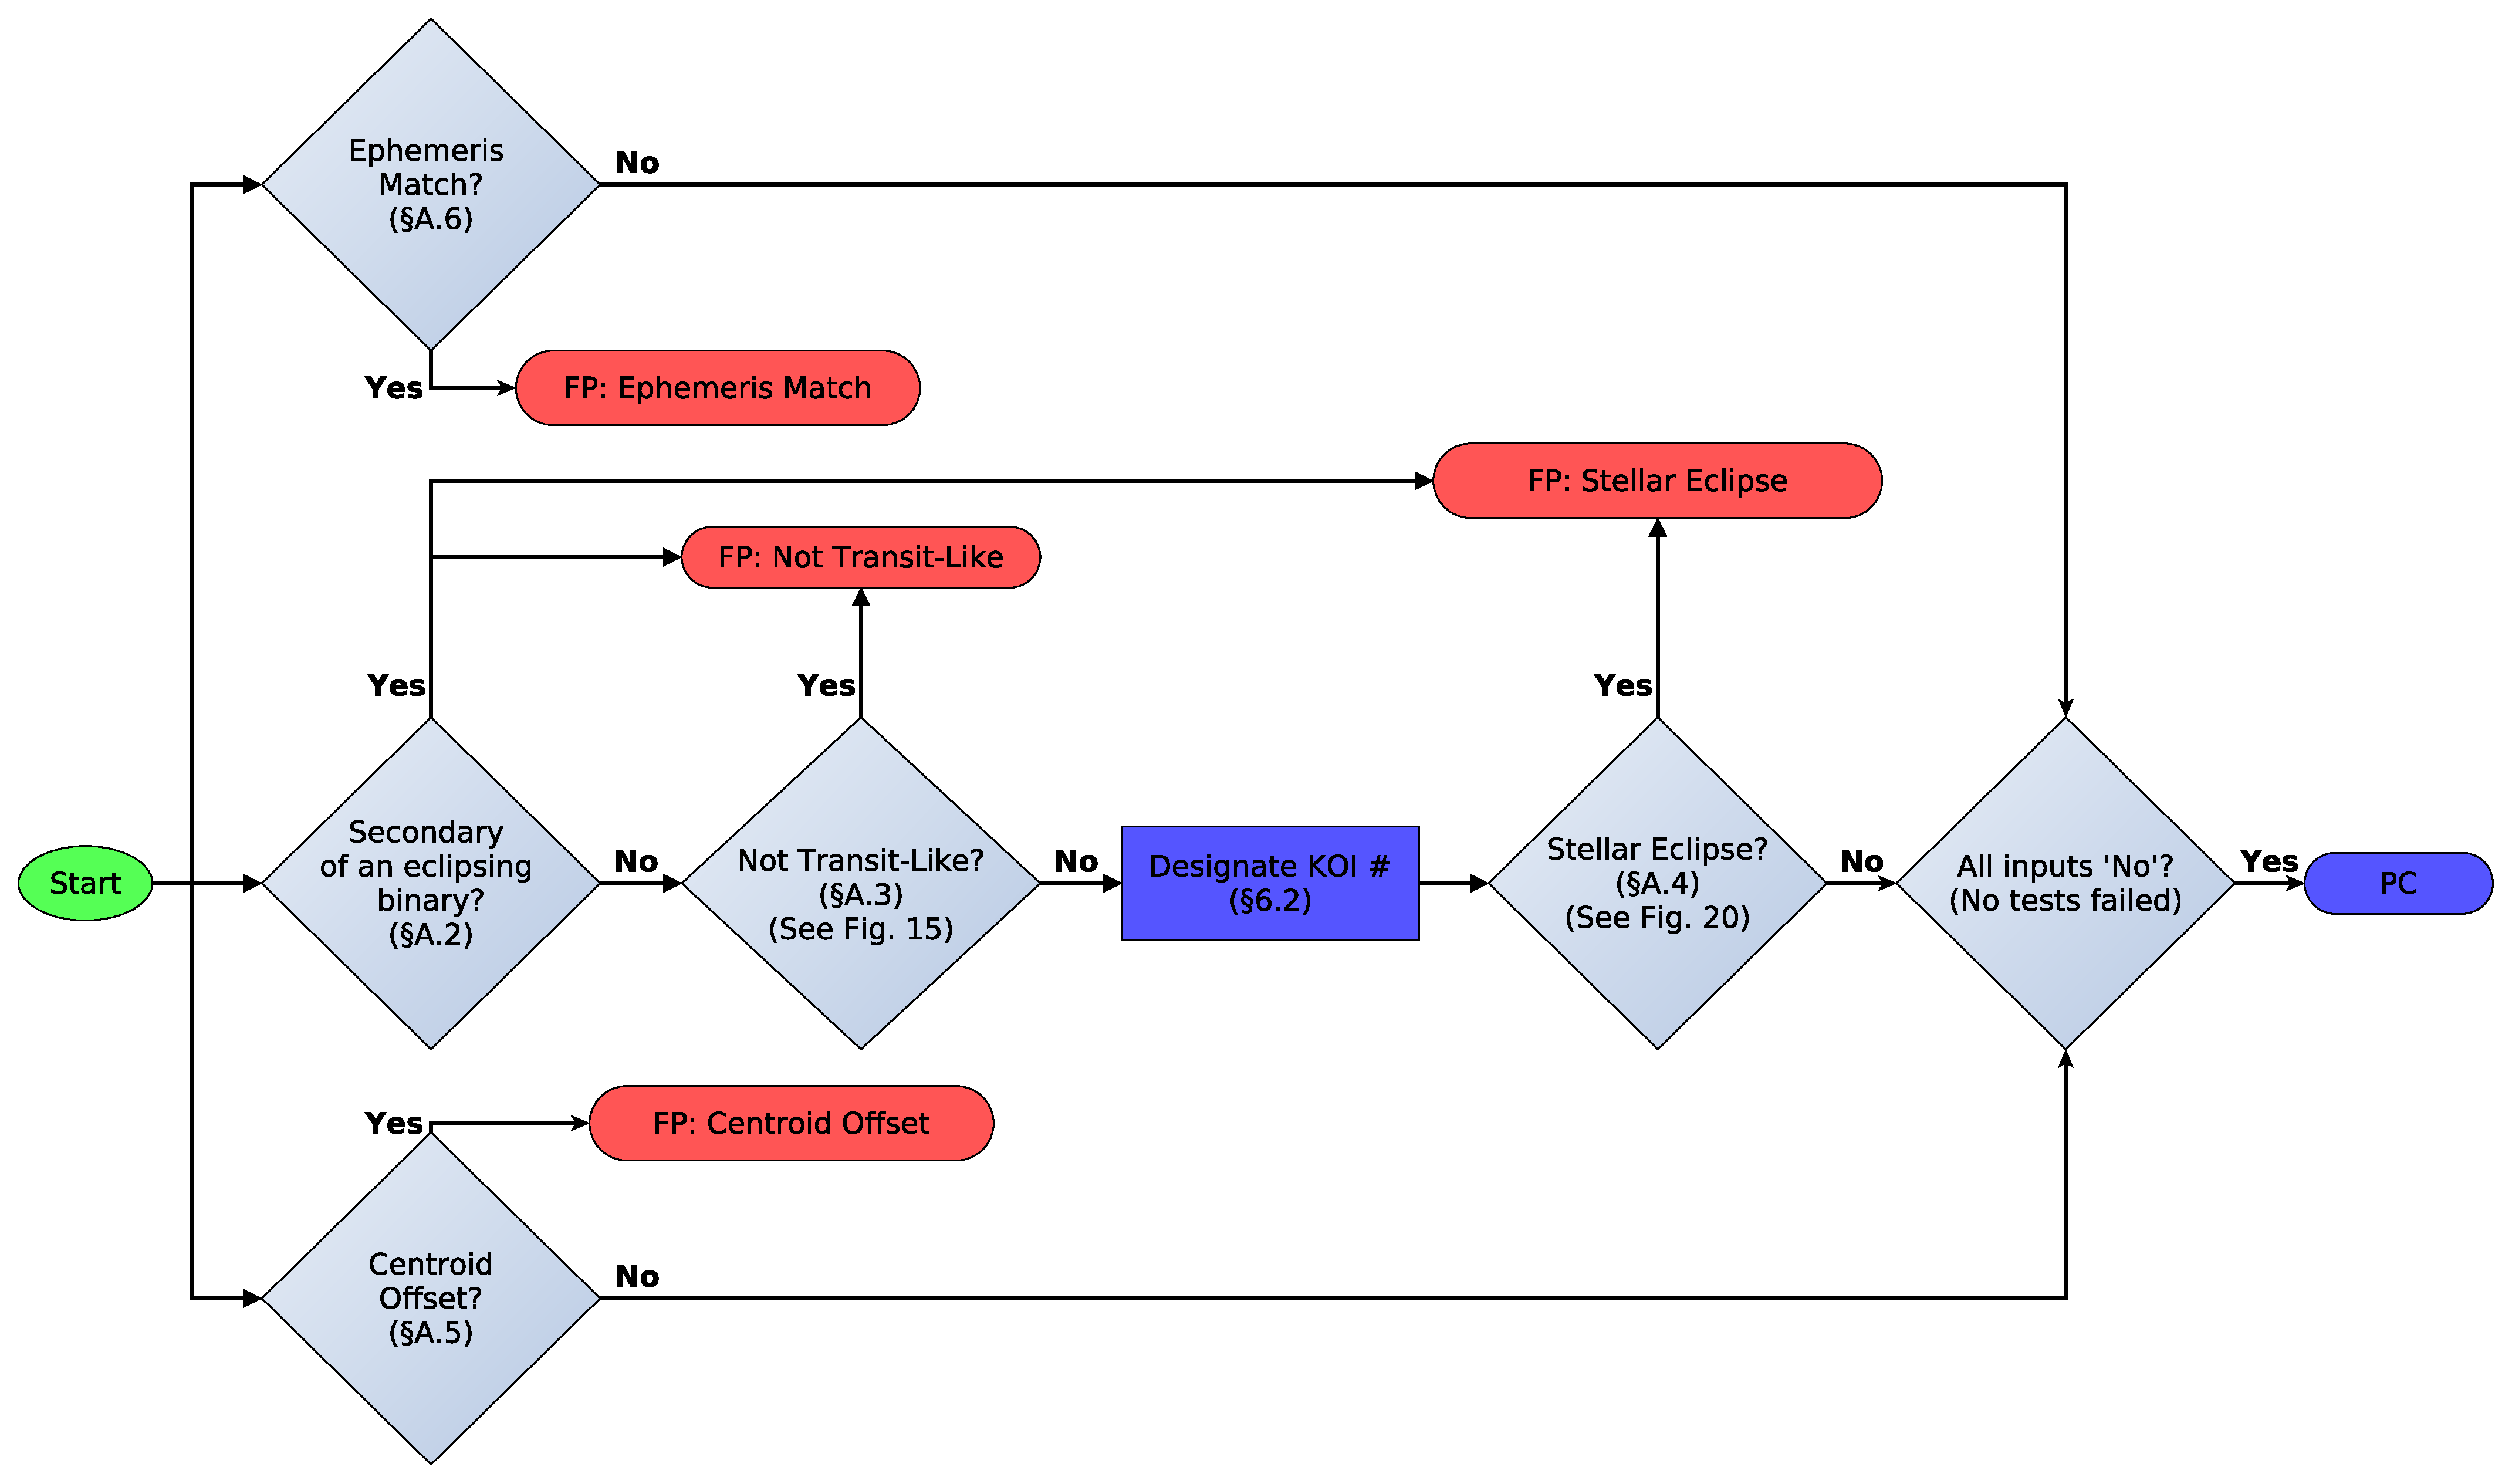
\includegraphics[width=0.9\linewidth]{RoboVetter-Diagram-V4-Overview.pdf}
\caption{Overview flowchart of the robovetter. Diamonds represent ``yes'' or ``no'' decisions that are made with quantitative metrics. A TCE is dispositioned as a FP if it fails any test (a ``yes'' decision) and is placed in one or more of the FP categories. (TCEs that are identified as being the secondary eclipses are placed in both the `Not Transit-Like' and 'Stellar Eclipse' categories.) If a TCE passes all tests (a ``no'' decision for all tests) it is dispositioned as a PC. The section numbers on each component correspond to the sections in this paper where these tests are discussed. More in-depth flowcharts are provided for the not transit-like and significant secondary modules in Figures~\ref{robovetter-transitlike-fig} and \ref{robovetter-sigsec-fig}.}
\label{robovetter-overview-fig}
\end{figure*}


The Robovetter first checks if the TCE corresponds to a secondary eclipse associated with a already examined TCE in that system. If not, the Robovetter then checks if the TCE is transit-like. If it is transit-like, the Robovetter then looks for the presence of a secondary eclipse. In parallel, the Robovetter also looks for evidence of a centroid offset and an ephemeris match to other TCEs and variable stars in the \kepler{} field. 

\label{s:majorflags}
Similar to previous KOI catalogs \citep{Rowe2015cat, Mullally2015cat, Coughlin2016}, the Robovetter assigns FP TCEs to one or more of the following false positive categories:


\begin{itemize}
  \item Not Transit-Like (NT): a TCE whose light curve is not consistent with that of a transiting planet or eclipsing binary, such as instrumental artifacts and non-eclipsing variable stars. Those TCEs  with only the Not Transit Like flag set are how the Robovetter signifies false alarms as we have defined them in this paper. 
  \item  Stellar Eclipse (SS): a TCE that is observed to have a significant secondary event, v-shaped transit profile, or out-of-eclipse variability that indicates the transit-like event is most likely caused by an eclipsing binary. Self-luminous, hot Jupiters with a visible secondary eclipse are also in this category, but are still given a disposition of PC. (In previous KOI catalogs this flag was known as Significant Secondary.)
  \item Centroid Offset (CO): a TCE whose signal is observed to originate on a nearby star, rather than the target star, based on examination of the pixel-level data.
  \item Ephemeris Match Indicates Contamination (EC): a TCE that has the same period and epoch as another object, and is not the true source of the signal given the relative magnitudes, locations, and signal amplitudes of the two objects. See \citet{Coughlin2014}.
\end{itemize}

The specific tests that caused the TCE to fail that category are given by minor flags. These flags are described in Appendix~\ref{s:minorflags}) and are available for all FPs.  Table~\ref{t:metrics} gives a summary of the specific tests run by the Robovetter when evaluating a TCE.  The table lists the false positive category (NT,SS, CO or EC) of the test and also which minor flags are set by that test.  Note that there are several informative minor flags, which are listed in Appendix~\ref{s:minorflags}, but are not listed in Table~\ref{t:metrics} because they do not change the disposition of a TCE.

New to this Robovetter are several tests that look at individual transits. The tests are named after the code that calculates the relevant metric and are called: Rubble, Marshall, Chases, Skye, Zuma and Tracker.  Each metric only identifies which transits can be considered ``bad", or not sufficiently transit-like.  The Robovetter then fails the TCE if the number of remaining good transits is less than three, or if the recalculated MES, using only the good transits, drops below 7.1.

Another note-worthy change to the DR25 Robovetter is the introduction of the v-shape metric, originally used in \citet{Batalha2013}.  The intent is to remove likely eclipsing binaries which do not show significant secondary eclipses by looking at the shape of the transit, see \S\ref{s:shapemetric}.

\begin{deluxetable*}{llcll}
\tablecolumns{11}
\tabletypesize{\scriptsize}
\tablewidth{\linewidth}
\tablecaption{Summary of the DR25 Robovetter tests}
\tablehead{
Test Name & Section & Major & Minor & Brief\\[-3pt]
                    &                   & Flags   & Flags & Description
        }
\startdata
Is Secondary    & \ref{s:issecond}  & \makecell{\\NT \\SS}  & IS\_SEC\_TCE                      & The TCE is a secondary eclipse.\\
\tableline\\[-4pt]
LPP Metric      & \ref{s:lpp}       & NT                & \makecell[l]{LPP\_DV \\ LPP\_ALT} & The TCE is not transit-shaped.\\[3pt]
\tableline\\[-4pt]
SWEET NTL       & \ref{s:sweetntl}  & NT                & SWEET\_NTL          & The TCE is sinusoidal.\\
\tableline\\[-4pt]
TCE Chases      & \ref{s:tcechases} & NT                & ALL\_TRANS\_CHASES  & The individual TCE events are not uniquely significant.\\[3pt]
\tableline\\[-4pt]
MS$_1$       & \ref{s:ms}           &  NT               & \makecell[l]{MOD\_NONUNIQ\_DV \\ MOD\_NONUNIQ\_ALT}   & The TCE is not significant compared to red noise.\\[2pt]
\tableline\\[-4pt]
MS$_2$      & \ref{s:ms}            & NT                & \makecell[l]{MOD\_TER\_DV\  \\ MOD\_TER\_ALT}     & Negative event in phased flux as significant as TCE.\\[3pt]
\tableline\\[-4pt]
MS$_3$      & \ref{s:ms}            & NT                & \makecell[l]{MOD\_POS\_DV \\MOD\_POS\_ALT}       & Positive event in phased flux as significant as TCE.\\[3pt]
\tableline\\[-4pt]
Max SES to MES                & \ref{s:sesmes}                    & NT                  & INCONSISTENT\_TRANS & The TCE is dominated by a single transit event.\\[3pt]
\tableline\\[-4pt]
Same Period                   & \ref{s:sameperiod}                & NT                  & SAME\_NTL\_PERIOD   & Has same period as a previous not transit-like TCE.\\[3pt]
\tableline\\[-4pt]
Individual Transits           & \ref{s:indivtrans}                & NT                  & INDIV\_TRANS\_      & Has $<$~3 good transits and recalculated MES $<$~7.1.\\[2pt]
\hspace{2em}Rubble            & \ref{s:rubble}                    & \nodata             & INDIV\_TRANS\_RUBBLE   & Transit does not contain enough cadences.\\
\hspace{2em}Marshall          & \ref{s:marshall}                  & \nodata             & INDIV\_TRANS\_MARSHALL & Transit shape more closely matches a known artifact. \\
\hspace{2em}Chases            & \ref{s:chases}                    & \nodata             & INDIV\_TRANS\_CHASES   & Transit event is not significant.\\[2pt]
\hspace{2em}Skye              & \ref{s:skye}                      & \nodata             & INDIV\_TRANS\_SKYE     & Transit time is correlated with other TCE transits. \\
\hspace{2em}Zuma              & \ref{s:zuma}                      & \nodata             & INDIV\_TRANS\_ZUMA     & Transit is consistent with an increase in flux.\\[2pt]
\hspace{2em}Tracker           & \ref{s:tracker}                   & \nodata             & INDIV\_TRANS\_TRACKER  & No match between fitted and discovery transit time.\\
\tableline\\[-4pt]
Gapped Transits               & \ref{s:rocky}                     & NT                  & TRANS\_GAPPED          &  The fraction of transits identified as bad is large.\\[3pt]
\tableline\\[-4pt]
MS Secondary & \ref{s:second}  & SS & \makecell[l]{MOD\_SEC\_DV \\  MOD\_SEC\_ALT} & A significant secondary event is detected.\\[2pt]
\tableline\\[-4pt]
Secondary TCE                 & \ref{s:secondTce}                 & SS & HAS\_SEC\_TCE  & A subsequent TCE on this star is the secondary.\\[3pt]
\tableline\\[-4pt]
Odd Even    & \ref{s:oddeven} & SS                      & \makecell[l]{DEPTH\_ODDEVEN\_DV \\ DEPTH\_ODDEVEN\_ALT \\MOD\_ODDEVEN\_DV \\MOD\_ODDEVEN\_ALT}  &  The depths of odd and even transits are different.\\[2pt]
\tableline\\[-4pt]
SWEET EB                      & \ref{s:sweeteb}                   & SS                  & SWEET\_EB           & Out-of-phase tidal deformation is detected.\\[3pt]
\tableline\\[-4pt]
V Shape Metric                & \ref{s:shapemetric}               & SS                  & DEEP\_V\_SHAPE      & The transit is deep and v-shaped.\\[3pt]
\tableline\\[-4pt]
Planet Occultation\tablenotemark{\tiny{PC}} & \ref{s:sscand} & SS & \makecell[l]{PLANET\_OCCULT\_DV \\PLANET\_OCCULT\_ALT}  & Significant secondary could be planet occultation.\\
\tableline\\[-4pt]
Planet Half Period\tablenotemark{\tiny{PC}} & \ref{s:sscand} & \nodata & \makecell[l]{PLANET\_PERIOD\_IS\_HALF\_DV \\ PLANET\_PERIOD\_IS\_HALF\_ALT}  &Planet scenario possible at half the DV period.\\[2pt]
\tableline\\[-4pt]
Resolved Offset               & \ref{s:centroidrv}                & CO                  & CENT\_RESOLVED\_OFFSET & The transit occurs on a spatially resolved target.\\[3pt]
\tableline\\[-4pt]
Unresolved Offset             & \ref{s:centroidrv}                & CO                  & CENT\_UNRESOLVED\_OFFSET & A shift in the centroid position occurs during transit.\\[3pt]
\tableline\\[-4pt]
Ghost Diagnostic              & \ref{s:ghost}                     & CO                  & HALO\_GHOST           & The transit strength in the halo pixels is too large.\\[3pt]
\tableline\\[-4pt]
Ephemeris Match               & \ref{s:ephemmatch}                & EC                  & EPHEM\_MATCH          & The ephemeris matches that of another source.\\
\enddata
\tablecomments{More details about all of these tests and how they are used by the Robovetter can be found in the sections listed in the second column.}
\label{t:metrics}
\tablenotetext{PC}{\hspace{1em}These tests override previous tests and will cause the TCE to become a planet candidate.}
\end{deluxetable*}


%Saving Old when switched to makecell.
% \begin{deluxetable*}{llcll}
% \tablecolumns{11}
% \tabletypesize{\scriptsize}
% \tablewidth{\linewidth}
% \tablecaption{Summary of the DR25 Robovetter tests}
% \tablehead{
% Test Name & Section & Major & Minor & Brief\\
%                     &                   & Flags   & Flags & Description
%         }
% \startdata
% \multirow{2}{*}{Is Secondary} & \multirow{2}{*}{\ref{s:issecond}} & NT & \multirow{2}{*}{IS\_SEC\_TCE}        & \multirow{2}{*}{The TCE is a secondary eclipse.}\\
%                               &                                   & SS &                                      & \\[1pt]
% \hline\\[-3pt]
% \multirow{2}{*}{LPP Metric}   & \multirow{2}{*}{\ref{s:lpp}}      & \multirow{2}{*}{NT} & LPP\_DV             & \multirow{2}{*}{The TCE is not transit-shaped.}\\[2pt]
%                               &                                   &                     & LPP\_ALT            & \\[3pt]
% \hline\\[-3pt]
% SWEET NTL                     & \ref{s:sweetntl}                  & NT                  & SWEET\_NTL          & The TCE is sinusoidal.\\[3pt]
% \hline\\[-3pt]
% TCE Chases                    & \ref{s:tcechases}                 & NT                  & ALL\_TRANS\_CHASES  & The individual TCE events are not significant.\\[3pt]
% \hline\\[-3pt]
% \multirow{2}{*}{MS$_1$}       & \multirow{2}{*}{\ref{s:ms}}       & \multirow{2}{*}{NT} & MOD\_NONUNIQ\_DV    & \multirow{2}{*}{The TCE is not significant compared to red noise.}\\[2pt]
%                               &                                   &                     & MOD\_NONUNIQ\_ALT   & \\[3pt]
% \hline\\[-3pt]
% \multirow{2}{*}{MS$_2$}       & \multirow{2}{*}{\ref{s:ms}}       & \multirow{2}{*}{NT} & MOD\_TER\_DV\       & \multirow{2}{*}{Negative event in phased flux as significant as TCE.}\\[2pt]
%                               &                                   &                     & MOD\_TER\_ALT       & \\[3pt]
% \hline\\[-3pt]
% \multirow{2}{*}{MS$_3$}       & \multirow{2}{*}{\ref{s:ms}}       & \multirow{2}{*}{NT} & MOD\_POS\_DV        & \multirow{2}{*}{Positive event in phased flux as significant as TCE.}\\[2pt]
%                               &                                   &                     & MOD\_POS\_ALT       & \\[3pt]
% \hline\\[-3pt]
% Max SES to MES                & \ref{s:sesmes}                    & NT                  & INCONSISTENT\_TRANS & The TCE is dominated by a single transit event.\\[3pt]
% \hline\\[-3pt]
% Same Period                   & \ref{s:sameperiod}                & NT                  & SAME\_NTL\_PERIOD   & Has same period as a previous not transit-like TCE.\\[3pt]
% \hline\\[-3pt]
% Individual Transits           & \ref{s:indivtrans}                & NT                  & INDIV\_TRANS\_      & Has $<$~3 good transits and recalculated MES $<$~7.1.\\[2pt]
% \hspace{2em}Rubble            & \ref{s:rubble}                    & \nodata             & INDIV\_TRANS\_RUBBLE   & Transit does not contain enough cadences.\\[2pt]
% \hspace{2em}Marshall          & \ref{s:marshall}                  & \nodata             & INDIV\_TRANS\_MARSHALL & Transit shape more closely matches a known artifact. \\[2pt]
% \hspace{2em}Chases            & \ref{s:chases}                    & \nodata             & INDIV\_TRANS\_CHASES   & Transit event is not significant.\\[2pt]
% \hspace{2em}Skye              & \ref{s:skye}                      & \nodata             & INDIV\_TRANS\_SKYE     & Transit time is correlated with other TCE transits. \\[2pt]
% \hspace{2em}Zuma              & \ref{s:zuma}                      & \nodata             & INDIV\_TRANS\_ZUMA     & Transit is consistent with an increase in flux.\\[2pt]
% \hspace{2em}Tracker           & \ref{s:tracker}                   & \nodata             & INDIV\_TRANS\_TRACKER  & No match between fitted and discovery transit time.\\[3pt]
% \hline\\[-3pt]
% Gapped Transits               & \ref{s:rocky}                     & NT                  & TRANS\_GAPPED          &  The fraction of transits identified as bad is large.\\[3pt]
% \hline\\[-3pt]
% \multirow{2}{*}{MS Secondary} & \multirow{2}{*}{\ref{s:second}}   & \multirow{2}{*}{SS} & MOD\_SEC\_DV  & \multirow{2}{*}{A significant secondary event is detected.}\\[2pt]
%                               &                                   &                     & MOD\_SEC\_ALT & \\[3pt]
% \hline\\[-3pt]
% Secondary TCE                 & \ref{s:secondTce}                 & SS & HAS\_SEC\_TCE  & A subsequent TCE on this star is the secondary.\\[3pt]
% \hline\\[-3pt]
% \multirow{4}{*}{Odd Even}     & \multirow{4}{*}{\ref{s:oddeven}}  & \multirow{4}{*}{SS} & DEPTH\_ODDEVEN\_DV  &  \multirow{4}{*}{The depths of odd and even transits are different.}\\[2pt]
%                               &                                   &                     & DEPTH\_ODDEVEN\_ALT & \\[2pt]
%                               &                                   &                     & MOD\_ODDEVEN\_DV    & \\[2pt]
%                               &                                   &                     & MOD\_ODDEVEN\_ALT   & \\[3pt]
% \hline\\[-3pt]
% SWEET EB                      & \ref{s:sweeteb}                   & SS                  & SWEET\_EB           & Out-of-phase tidal deformation is detected.\\[3pt]
% \hline\\[-3pt]
% V Shape Metric                & \ref{s:shapemetric}               & SS                  & DEEP\_V\_SHAPE      & The transit is deep and v-shaped.\\[3pt]
% \hline\\[-3pt]
% \multirow{2}{*}{Planet Occultation\tablenotemark{\tiny{PC}}} & \multirow{2}{*}{\ref{s:sscand}} & \multirow{2}{*}{SS} & PLANET\_OCCULT\_DV & \multirow{2}{*}{Significant secondary could be planet occultation.}\\[2pt]
%                                                              &                                 &                     & PLANET\_OCCULT\_ALT & \\[3pt]
% \hline\\[-3pt]
% \multirow{2}{*}{Planet Half Period\tablenotemark{\tiny{PC}}} & \multirow{2}{*}{\ref{s:sscand}} & \multirow{2}{*}{\nodata} & PLANET\_PERIOD\_IS\_HALF\_DV & \multirow{2}{*}{Planet scenario possible at half the DV period.}\\[2pt]
%                                                              &                                 &                          & PLANET\_PERIOD\_IS\_HALF\_ALT & \\[3pt]
% \hline\\[-3pt]
% Resolved Offset               & \ref{s:centroidrv}                & CO                  & CENT\_RESOLVED\_OFFSET & The transit occurs on a spatially resolved target.\\[3pt]
% \hline\\[-3pt]
% Unresolved Offset             & \ref{s:centroidrv}                & CO                  & CENT\_UNRESOLVED\_OFFSET & A shift in the centroid position occurs during transit.\\[3pt]
% \hline\\[-3pt]
% Ghost Diagnostic              & \ref{s:ghost}                     & CO                  & HALO\_GHOST           & The transit strength in the halo pixels is too large.\\[3pt]
% \hline\\[-3pt]
% Ephemeris Match               & \ref{s:ephemmatch}                & EC                  & EPHEM\_MATCH          & The ephemeris matches that of another source.\\[-7pt]
% \enddata
% \tablecomments{More details about all of these tests and how they are used by the Robovetter can be found in the sections listed in the second column.}
% \label{t:metrics}
% \tablenotetext{PC}{These tests override previous tests and will cause the TCE to become a planet candidate.}
% \end{deluxetable*}


% Saving Old Table Before Jeff Edits
% 
% \begin{deluxetable*}{lllll}

% \tablecolumns{11}
% \tabletypesize{\scriptsize}
% \tablewidth{\linewidth}
% \tablecaption{Summary of the DR25 Robovetter tests}
% \tablehead{Test Name & Section & \spcell{Major\\Flags} & \spcell{Minor\\Flags} & \spcell{Brief\\Description} }
% \startdata

% Is Secondary  & \ref{s:issecond} & \spcell{NT\\SS} & IS\_SEC\_TCE & The TCE is a secondary eclipse\\
% \hline\\
% LPP Metric    & \ref{s:lpp}      & NT   & \spcell{LPP\_DV\\LPP\_ALT} & The folded event is transit-shaped. \\
% \hline\\
% SWEET NTL     & \ref{s:sweetntl} & NT   &  \spcell{SWEET\_NTL}                & The folded event is sinusoidal. \\[2pt]
% \hline\\
% TCE Chases    &  \ref{s:tcechases} & NT & ALL\_TRANS\_CHASES         & The indiv. transit detection statistics are unique. \\[2pt]
% \hline\\
% MS$_1$        &   \ref{s:ms}       & NT & \spcell{MOD\_NONUNIQ\_DV\\MOD\_NONUNIQ\_ALT} & The folded transit is significant compared to red noise.  \\
% \hline\\
% MS$_2$        &  \ref{s:ms}        & NT & \spcell{MOD\_TER\_DV\\MOD\_TER\_ALT} & Other phases are significant in the folded light curve. \\
% \hline\\
% MS$_3$        & \ref{s:ms}         & NT & \spcell{MOD\_POS\_DV\\MOD\_POS\_ALT} & Significant positive going event in the folded light curve.  \\
% \hline\\
% Max SES to MES &  \ref{s:sesmes}  & NT & INCONSISTENT\_TRANS          & Dominated by a single transit. \\[2pt]
% \hline\\
% Same Period    & \ref{s:sameperiod} & NT &  SAME\_NTL\_PERIOD       & Same period as a previous not-transit-like TCE. \\[2pt]
% \hline\\
% Individual Transits & \ref{s:indivtrans} & NT & INDIV\_TRANS\_ & Three transits remain whose recalculated MES is $\geq$7.1.\\[2pt]
% \hspace{2em}Rubble         & \ref{s:rubble}    & - & INDIV\_TRANS\_RUBBLE    & Transit does not contain enough cadences.\\
% \hspace{2em}Marshall       & \ref{s:marshall}   & - & INDIV\_TRANS\_MARSHALL  & Transit shape more closely matches a known artifact. \\
% \hspace{2em}Chases         & \ref{s:chases}     & - & INDIV\_TRANS\_CHASES    & Transit event is not uniquely significant.\\
% \hspace{2em}Skye           & \ref{s:skye}       & - & INDIV\_TRANS\_SKYE      & Transit time is correlated with other TCE transits. \\
% \hspace{2em}Zuma           & \ref{s:zuma}       & - & INDIV\_TRANS\_ZUMA      & Transit is consistent with an increase in flux.\\
% \hspace{2em}Tracker        & \ref{s:tracker}   & - & INDIV\_TRANS\_TRACKER   & Fitted transit time does not match discovery transit time.\\
% \hline\\
% Gapped Transits& \ref{s:rocky}     & NT & TRANS\_GAPPED          &  The fraction of transits identified as bad is large.\\
% \hline\\
% MS Secondary& \ref{s:second} & SS & \spcell{MOD\_SEC\_DV\\MOD\_SEC\_ALT} & A significant secondary event is detected. \\
% \hline\\
% Secondary TCE& \ref{s:secondTce} & SS & HAS\_SEC\_TCE & A subsequent TCE on the same star is the secondary.\\
% \hline\\
% Odd Even &  \ref{s:oddeven} & SS & \spcell{DEPTH\_ODDEVEN\_DV\\DEPTH\_ODDEVEN\_ALT\\MOD\_ODDEVEN\_DV\\MOD\_ODDEVEN\_ALT} &  The depth of odd and even transits is different.\\
% \hline\\
% SWEET EB & \ref{s:sweeteb} & SS & SWEET\_EB & Out-of-phase tidal deformation is detected.\\
% \hline\\
% V Shape Metric & \ref{s:shapemetric} & SS & DEEP\_V\_SHAPE & The transit is v-shaped.\\
% \hline\\
% Planet Occultation\tablenotemark{\tiny{PC}} & \ref{s:sscand} & SS & \spcell{PLANET\_OCCULT\_DV\\PLANET\_OCCULT\_ALT} & Significant secondary could be planet occultation.\\
% \hline\\
% Planet Half Period\tablenotemark{\tiny{PC}} & \ref{s:sscand} & -  & \spcell{PLANET\_PERIOD\_IS\_HALF\_DV\\PLANET\_PERIOD\_IS\_HALF\_ALT} & Planet scenario possible at half the DV period.\\
% \hline\\
% Resolved Offset & \ref{s:centroidrv} & CO & CENT\_RESOLVED\_OFFSET & The transit occurs on a spatially resolved target.\\
% \hline\\
% Unresolved Offset & \ref{s:centroidrv} & CO & CENT\_UNRESOLVED\_OFFSET & A shift in the centroid position occurs during transit.\\
% \hline\\
% Ghost Diagnostic & \ref{s:ghost} & CO & HALO\_GHOST & The transit strength in the halo pixels is too large.\\
% \hline\\
% Ephemeris Match & \ref{s:ephemmatch} & EC & EPHEM\_MATCH & The ephemeris matches that of another source.

% \enddata
% \tablecomments{More details about all of these tests and how they are used by the Robovetter can be found in 
% Appendix \ref{s:metrics}. }
% \label{t:metrics}
% \tablenotetext{PC}{These tests override previous tests and will cause the TCE to become a planet candidate.}
% \end{deluxetable*}

\subsection{Disposition Scores}
\label{s:scores}
We introduce a new feature to this catalog called the Disposition Score. Essentially the disposition score is a value between 0 and 1 that indicates the confidence in a disposition provided by the Robovetter. A higher value indicates more confidence that a TCE is a PC, regardless of the disposition it was given. This feature allows one to select the highest quality PCs by ranking KOIs via the disposition score, for both use in selecting samples for occurrence rate calculations and prioritizing individual objects for follow-up. \emph{We stress that the disposition score does not map directly to a probability that the signal is a planet.} However, in \S\ref{s:crscores} we discuss how the disposition score can be used to adjust the reliability of a sample.
%This statistics argument hasn't been proven. We could discuss this, but it belongs in the disucssion "and weight them appropriately for their statistics."

The disposition score was calculated by wrapping the Robovetter in a Monte Carlo routine. In each Monte Carlo iteration, for each TCE, new values are chosen for most of the Robovetter input metrics by drawing from an asymmetric Gaussian distribution centered on the nominal value. The Robovetter then dispositions each TCE given the new values for its metrics. The disposition score is simply the fraction of Monte Carlo iterations that result in a disposition of PC. (We used 10,000 iterations for the results in this catalog.) For example, if a TCE that is initially dispositioned as a PC has several metrics that are just barely on the passing side of their Robovetter thresholds, in many iterations at least one will be perturbed across the threshold. As a result, many of the iterations will produce a false positive and the TCE will be dispositioned as a PC with a low score.  Similarly, if a TCE only fails due to a single metric that was barely on the failing side of a threshold, the score may be near 0.5, indicating that it was deemed a PC in half of the iterations. Note that since a TCE is deemed a FP even if only one metric fails, nearly all FPs have scores less than 0.5, with most very close to 0.0.  PCs have a wider distribution of scores from 0.0 to 1.0 depending on how many of their metrics fall near to the various Robovetter thresholds.

To compute the asymmetric Gaussian distribution for each metric, we examined the metric distributions for the injected on-target planet population on FGK dwarf targets. We calculated a positive and negative median absolute deviation (MAD) value for each metric in a 20 by 20 grid in linear period space (ranging from 0.5 to 500 days) and logarithmic MES space (ranging from 7.1 to 100). We chose to use MAD because it is robust to outliers. MES and period were chosen as they are fundamental properties of a TCE that track each metric's variation. The MAD values were then multiplied by a conversion factor of 1.4826 to put the variability on the same scale as a Gaussian standard deviation \citep{Hampel1974,Ruppert2010}. A two-dimensional power-law was then fitted to the 20 by 20 grid of standard deviation values, separately for the positive and negative sigma directions. With this analytical approximation for a given metric, an asymmetrical Gaussian distribution can be generated for each metric for any TCE given its MES and period.

An example is shown in Figure~\ref{score-fig-1} for the LPP metric (Locality Preserving Projections, see \S\ref{s:lpp}) using the DV detrending. The top-left plot shows the LPP values of all on-target injected planets on FGK dwarf targets as a function of period, and the top-right shows them as a function of MES. The middle-left plots shows the measured positive 1$\sigma$ deviation (in the same units as the LPP metric) as a function of MES and period, and the middle-right plot shows the resulting best-fit model. The bottom plots show the same thing but for the negative 1$\sigma$ deviation. As can be seen, the scatter in the LPP metric has a weak period dependence, but a strong MES dependence, due to the fact it is easier to measure the overall shape of the light curve (LPP's goal) with higher MES (signal-to-noise). Also seen is that because LPP is bounded by zero on one side, LPP can scatter to very high values, especialy for low MES events. 

Most, but not all, of the Robovetter metrics were amenable to this approach. Specifically, the list of metrics that were perturbed in the manner above to generate the score values were: LPP (both DV and ALT), all the Model-shift metrics (both DV and ALT), TCE Chases, max-SES-to-MES, the two odd/even metrics (both DV and ALT), Ghost Diagnostic, and the recomputed MES using only good transits left after the individual transit metrics.

\begin{figure*}[hbtp]
\centering
\begin{tabular}{cc}
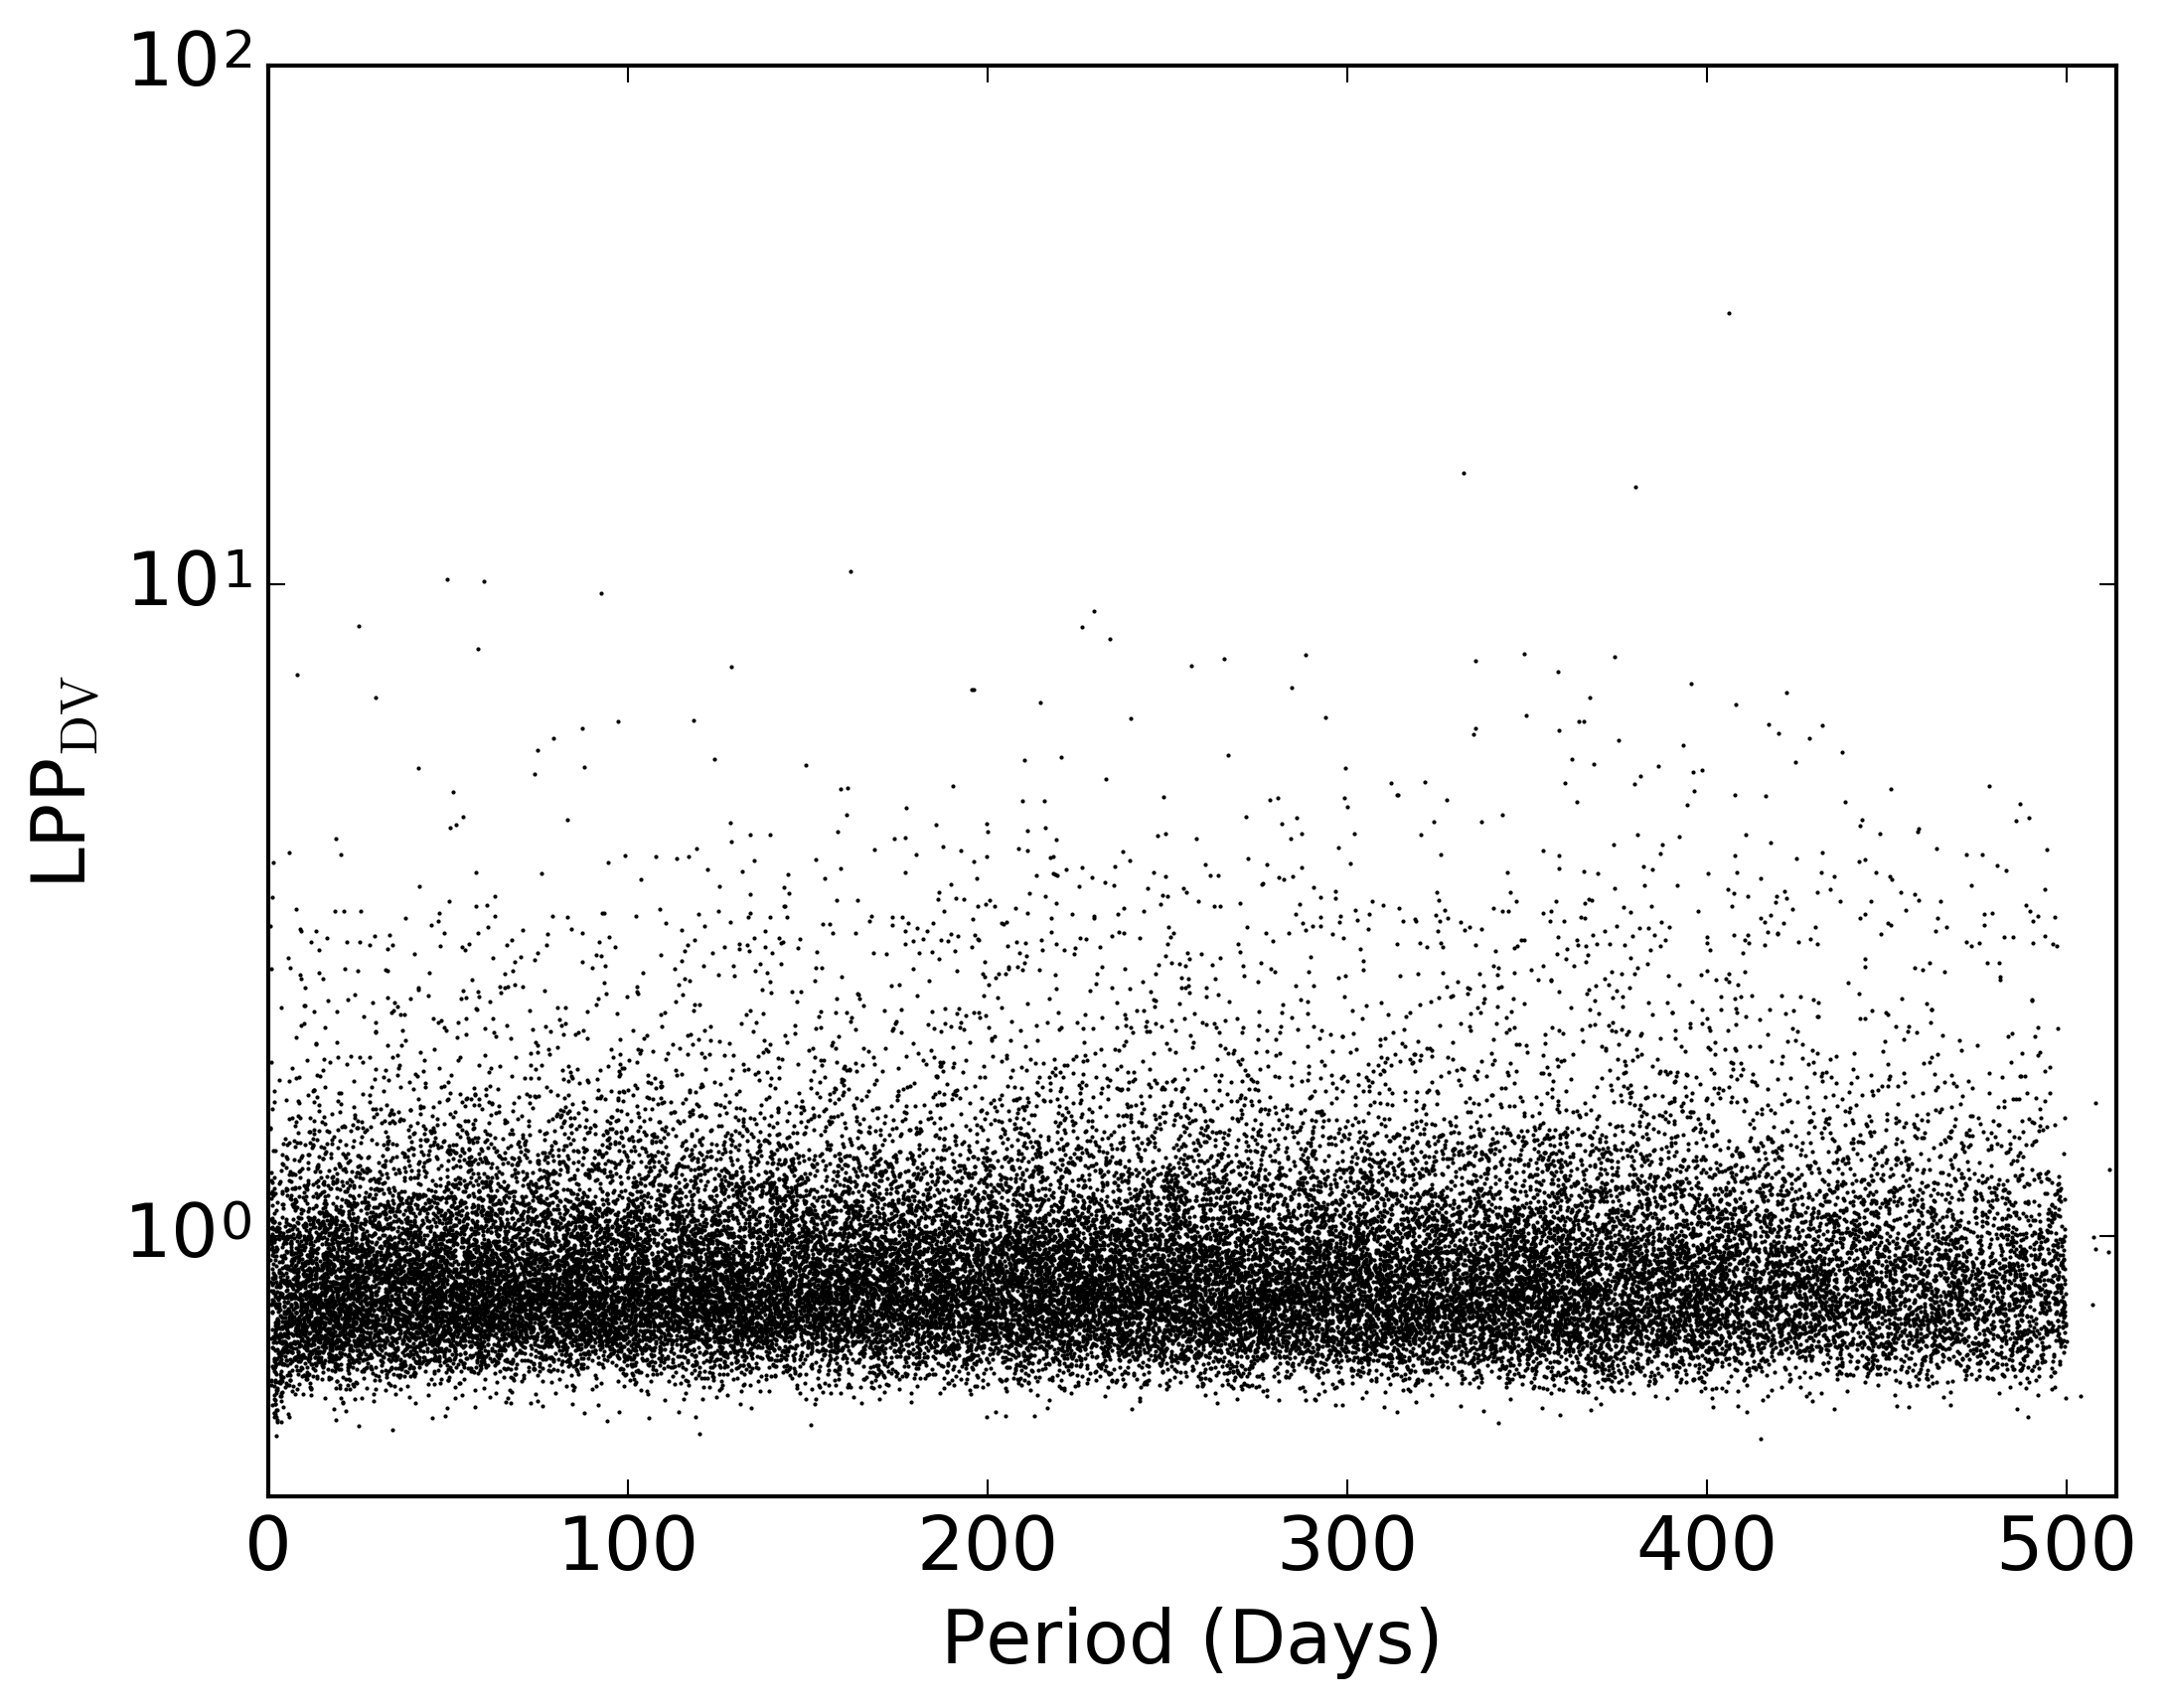
\includegraphics[width=0.5\linewidth]{ScoreFig-1.png} &
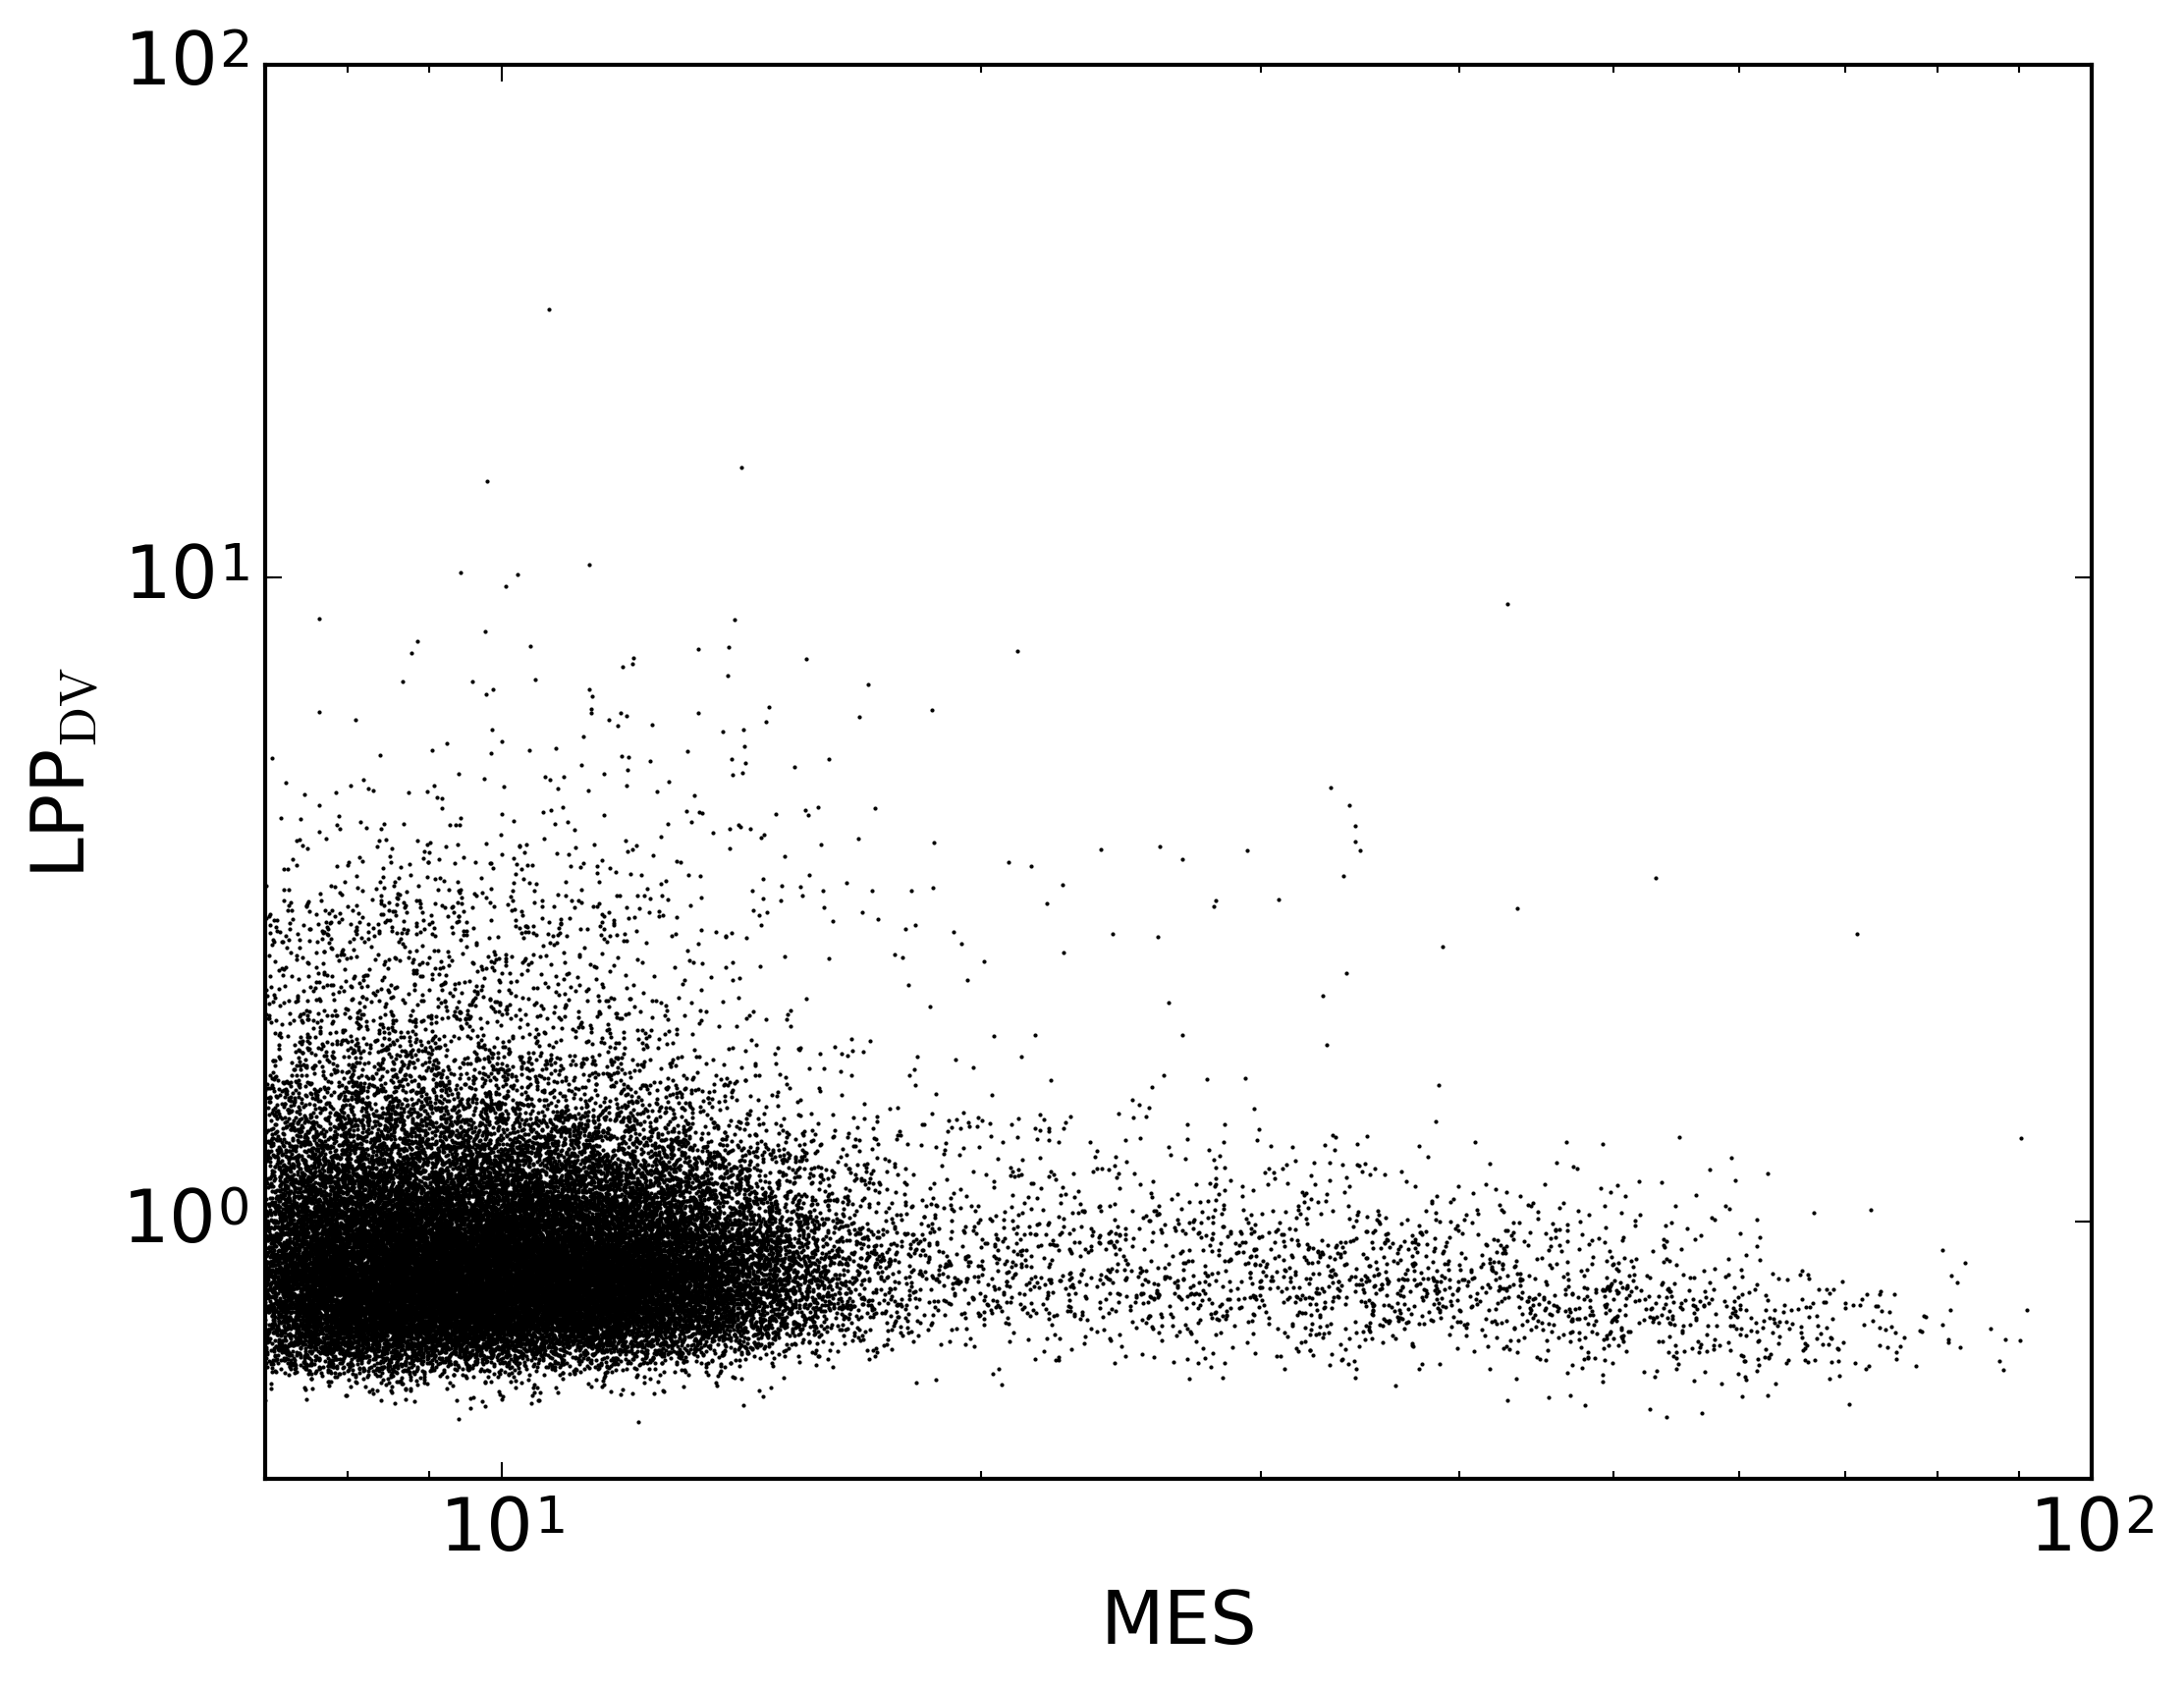
\includegraphics[width=0.5\linewidth]{ScoreFig-2.png} \\
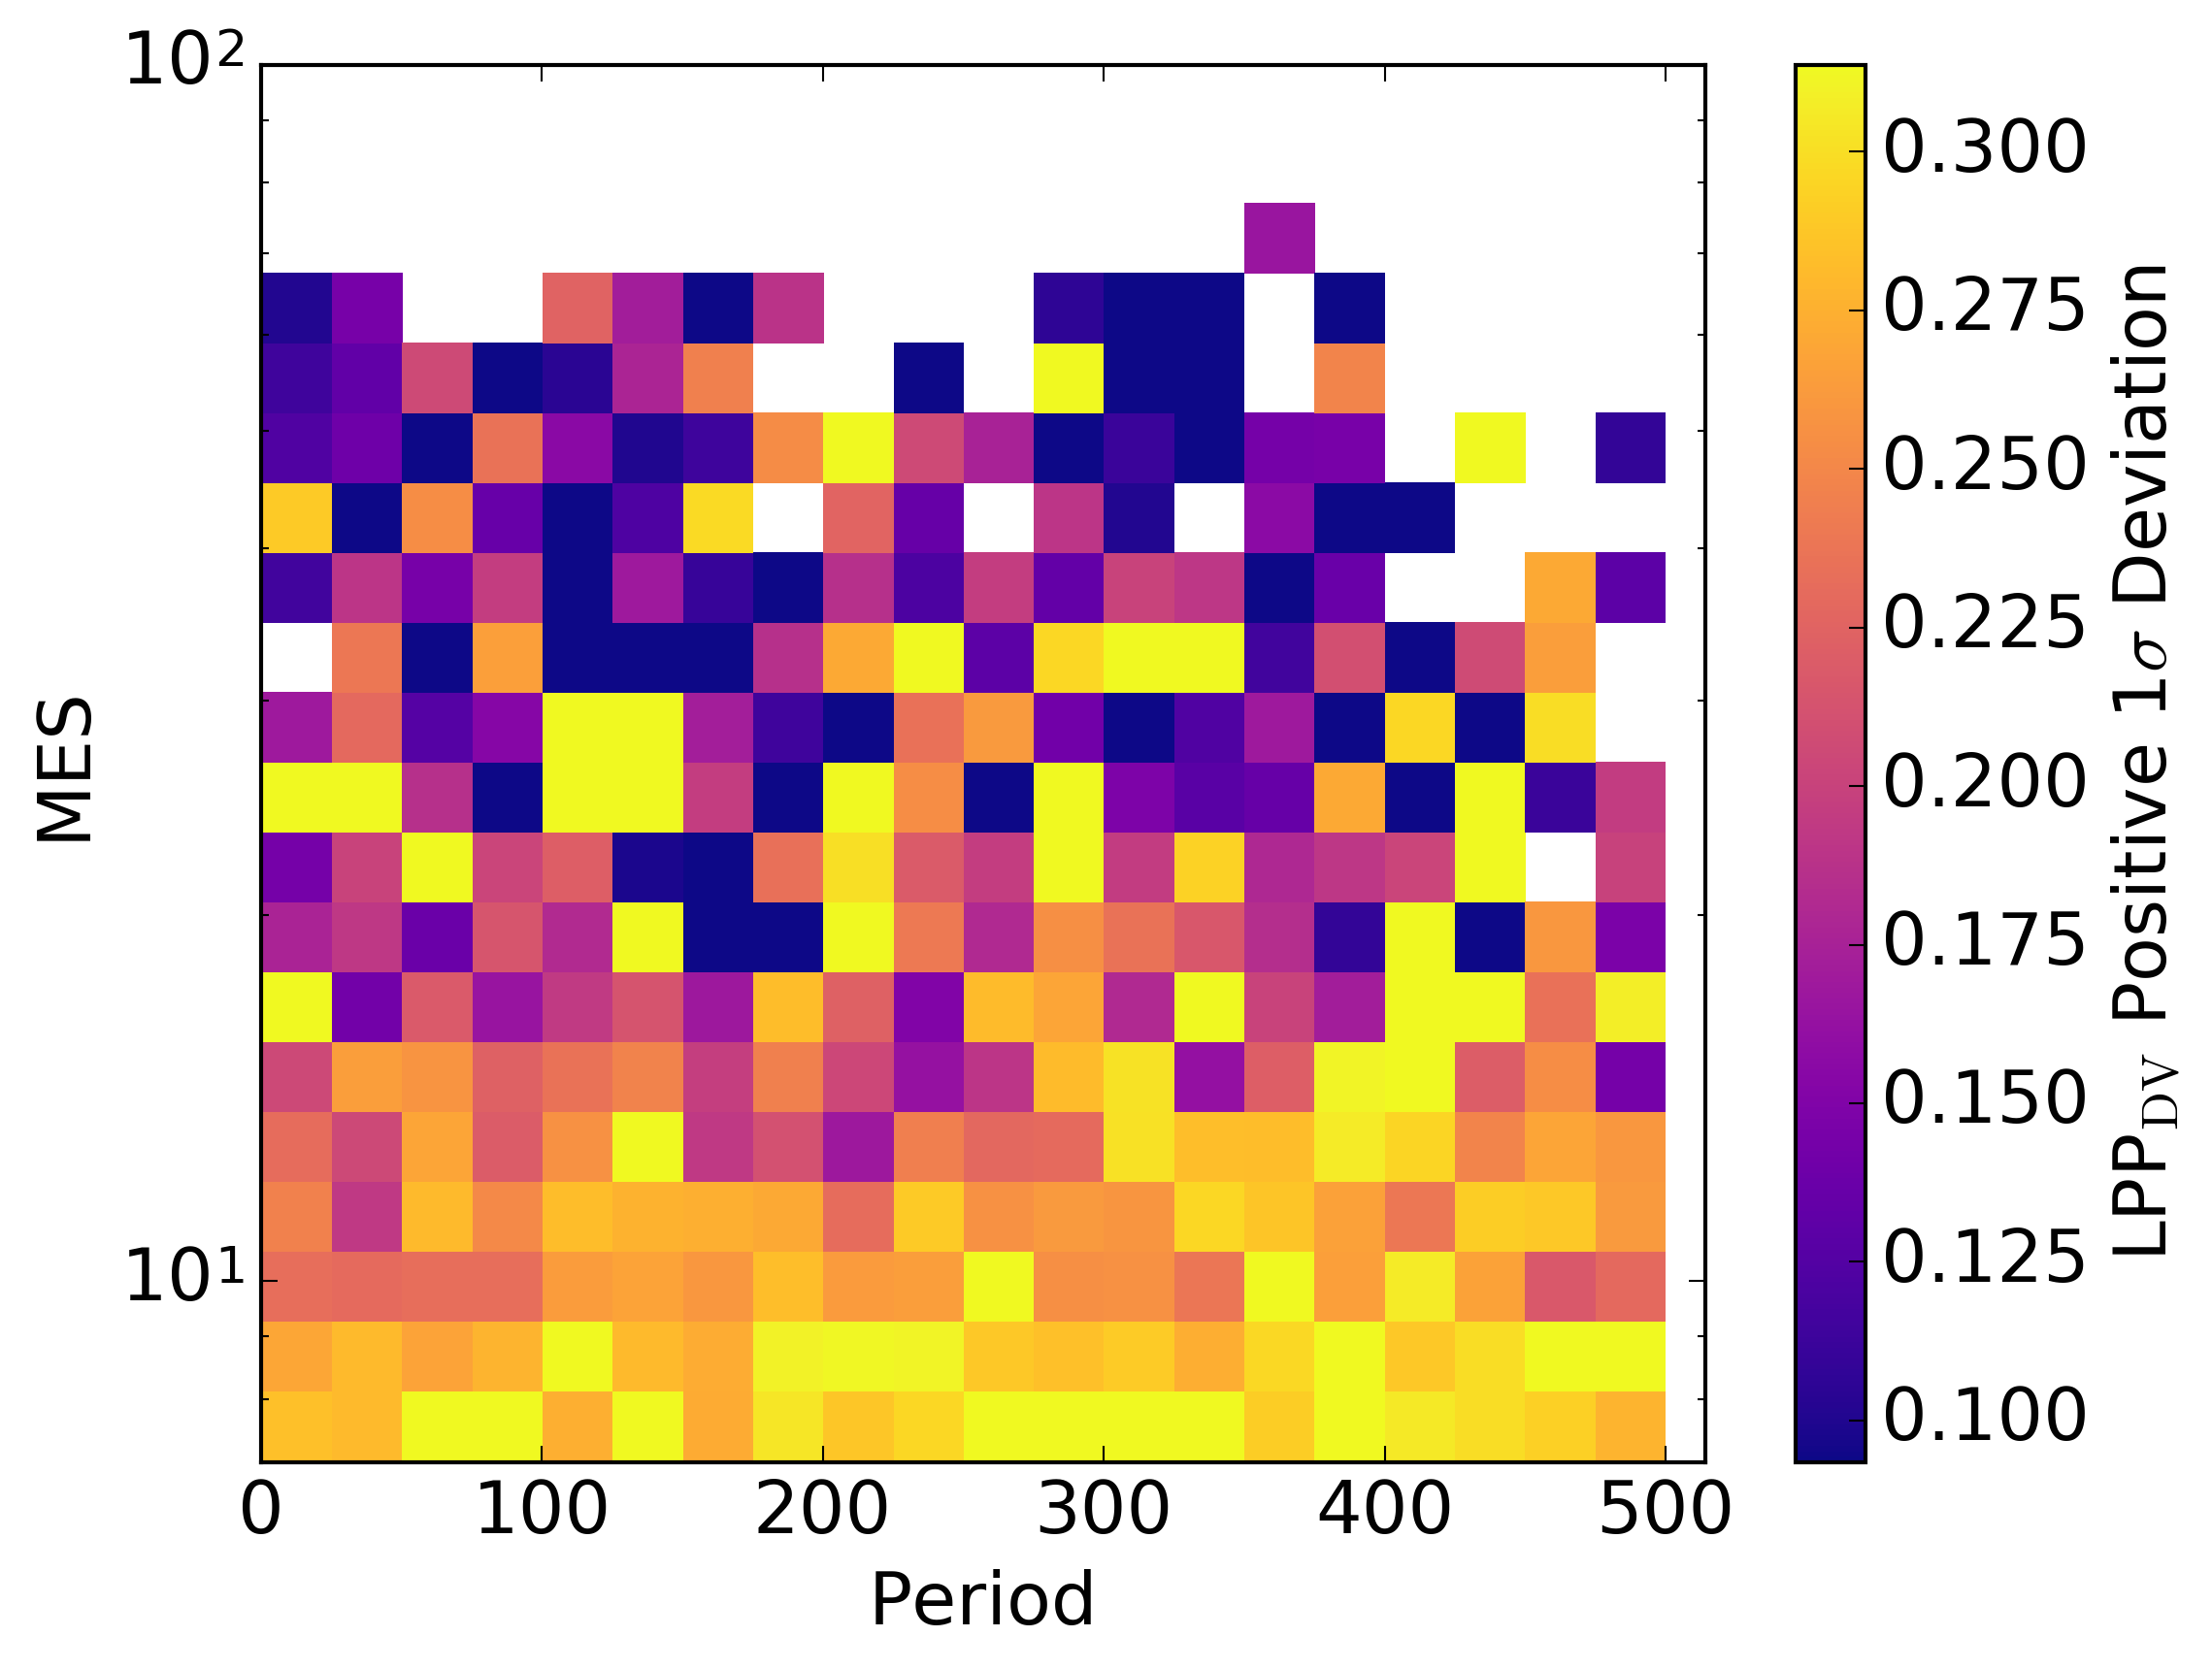
\includegraphics[width=0.5\linewidth]{ScoreFig-3.png} &
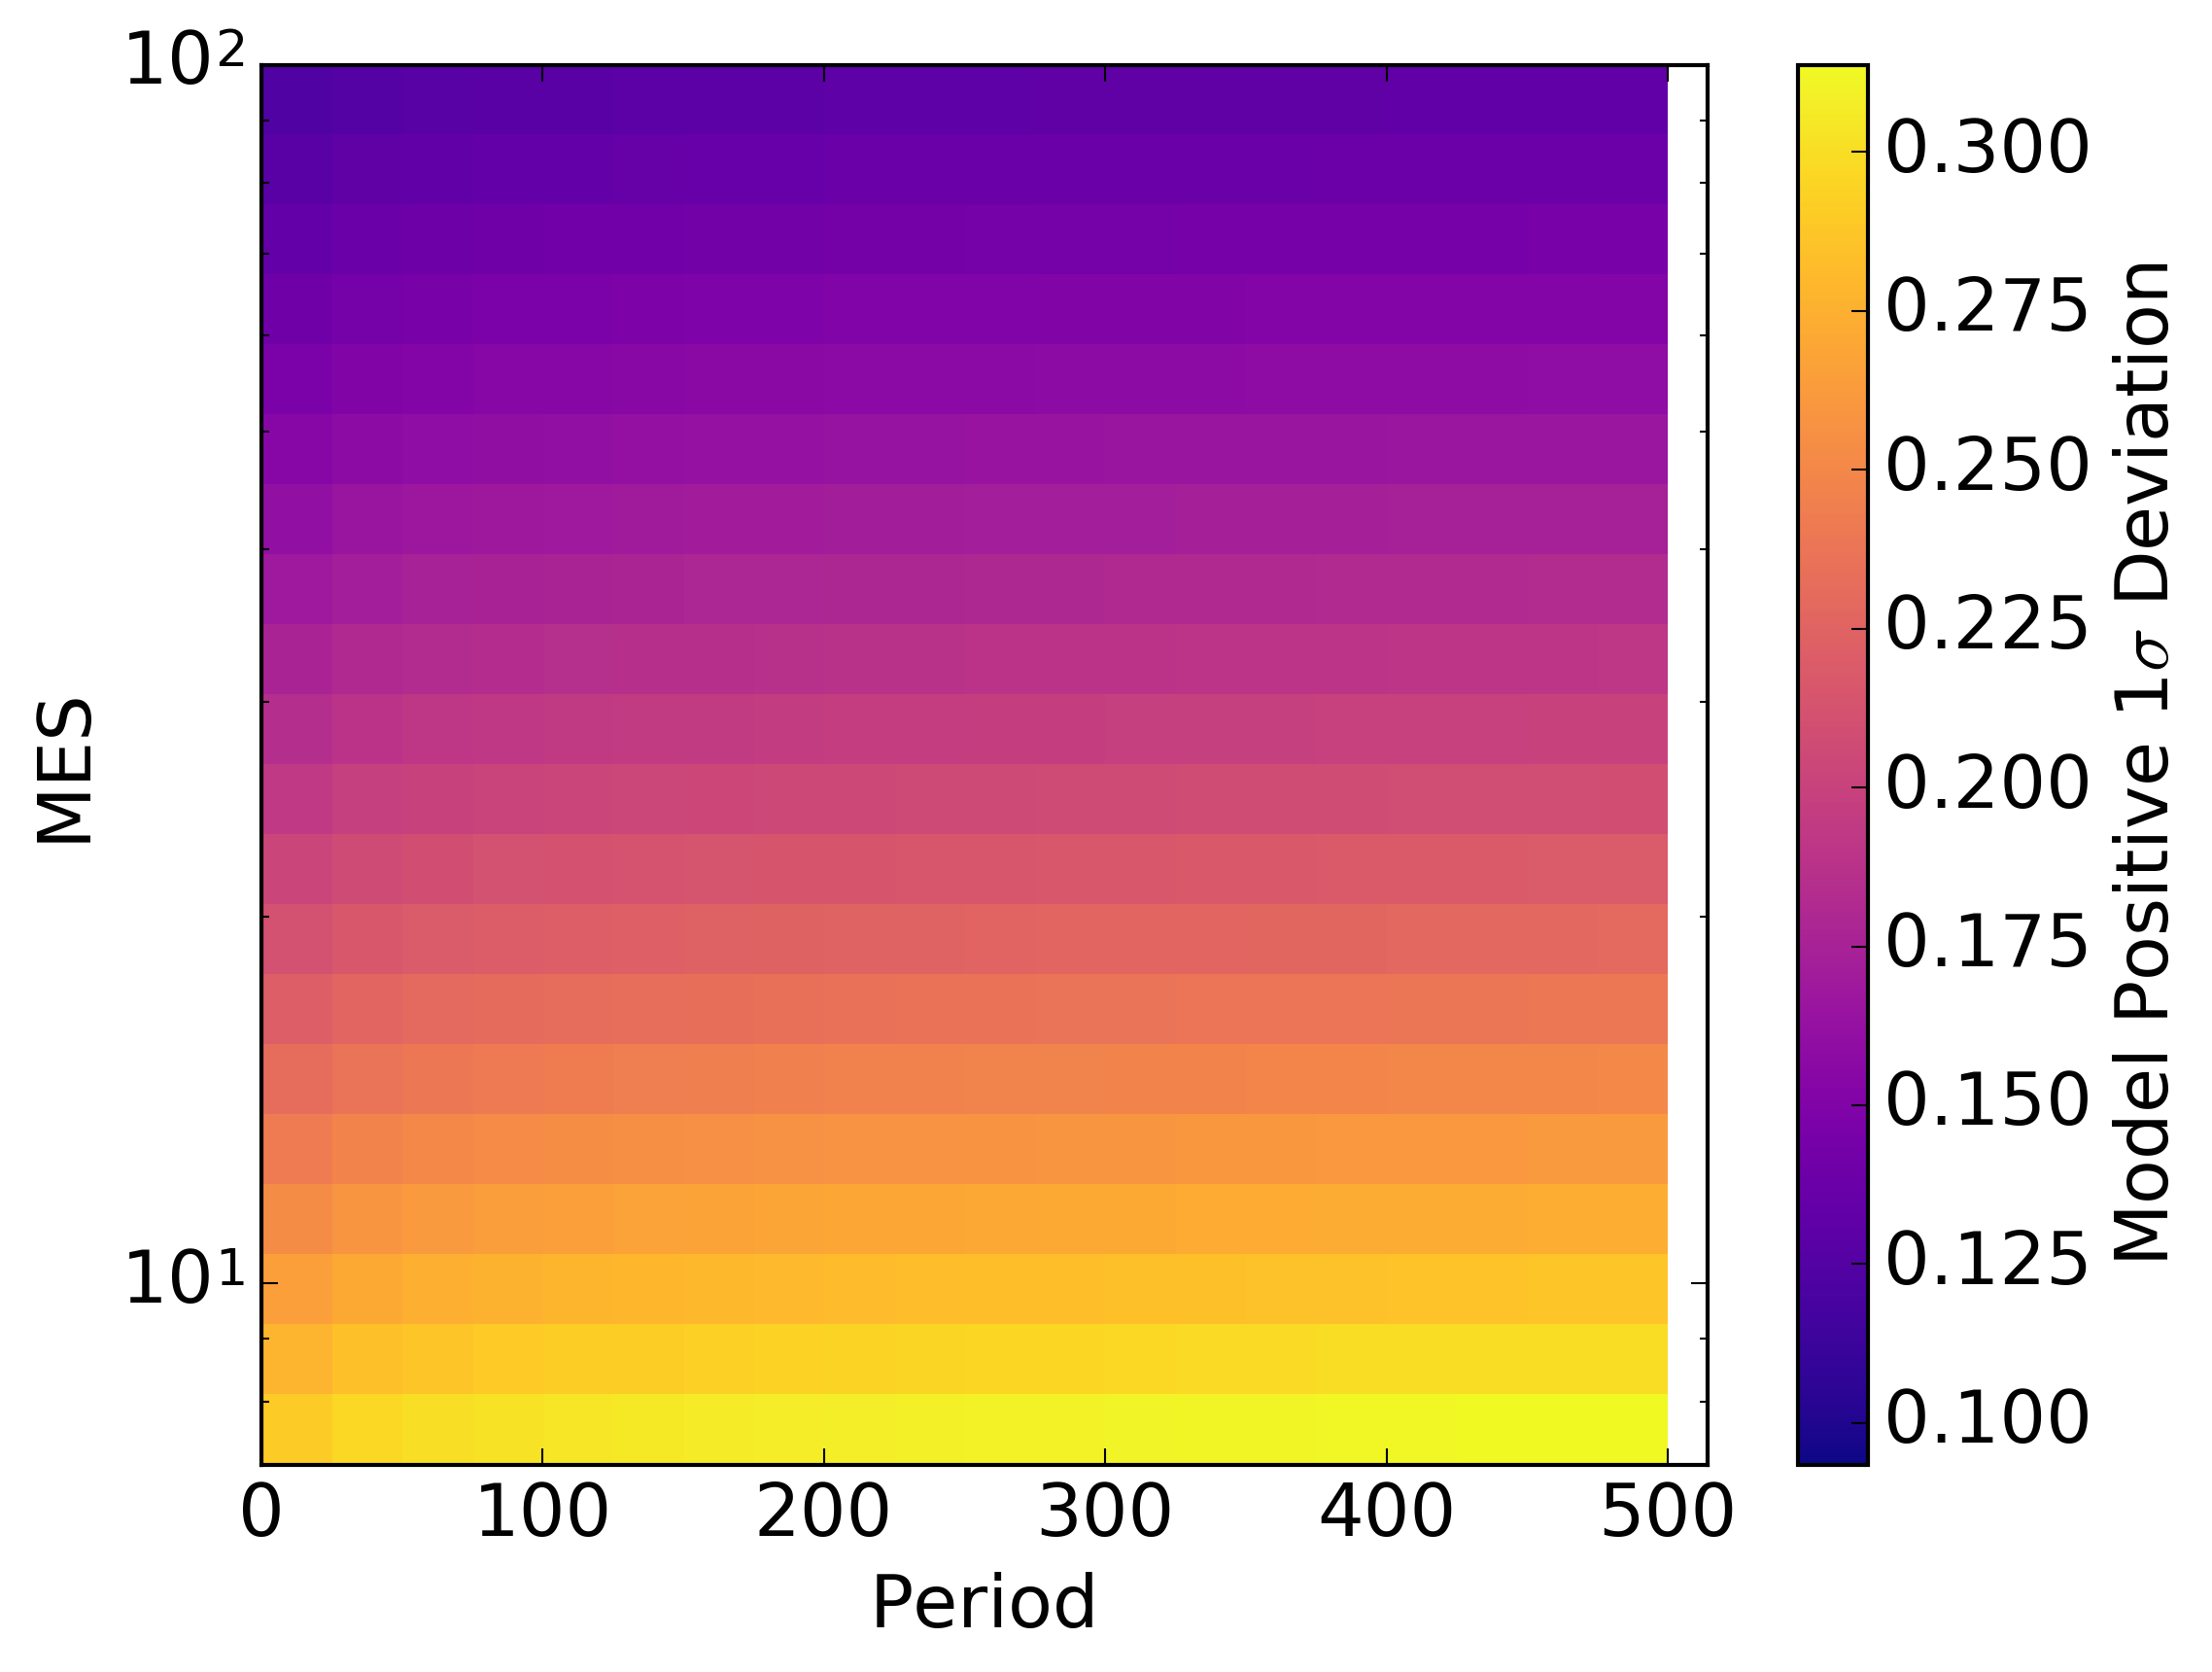
\includegraphics[width=0.5\linewidth]{ScoreFig-4.png} \\
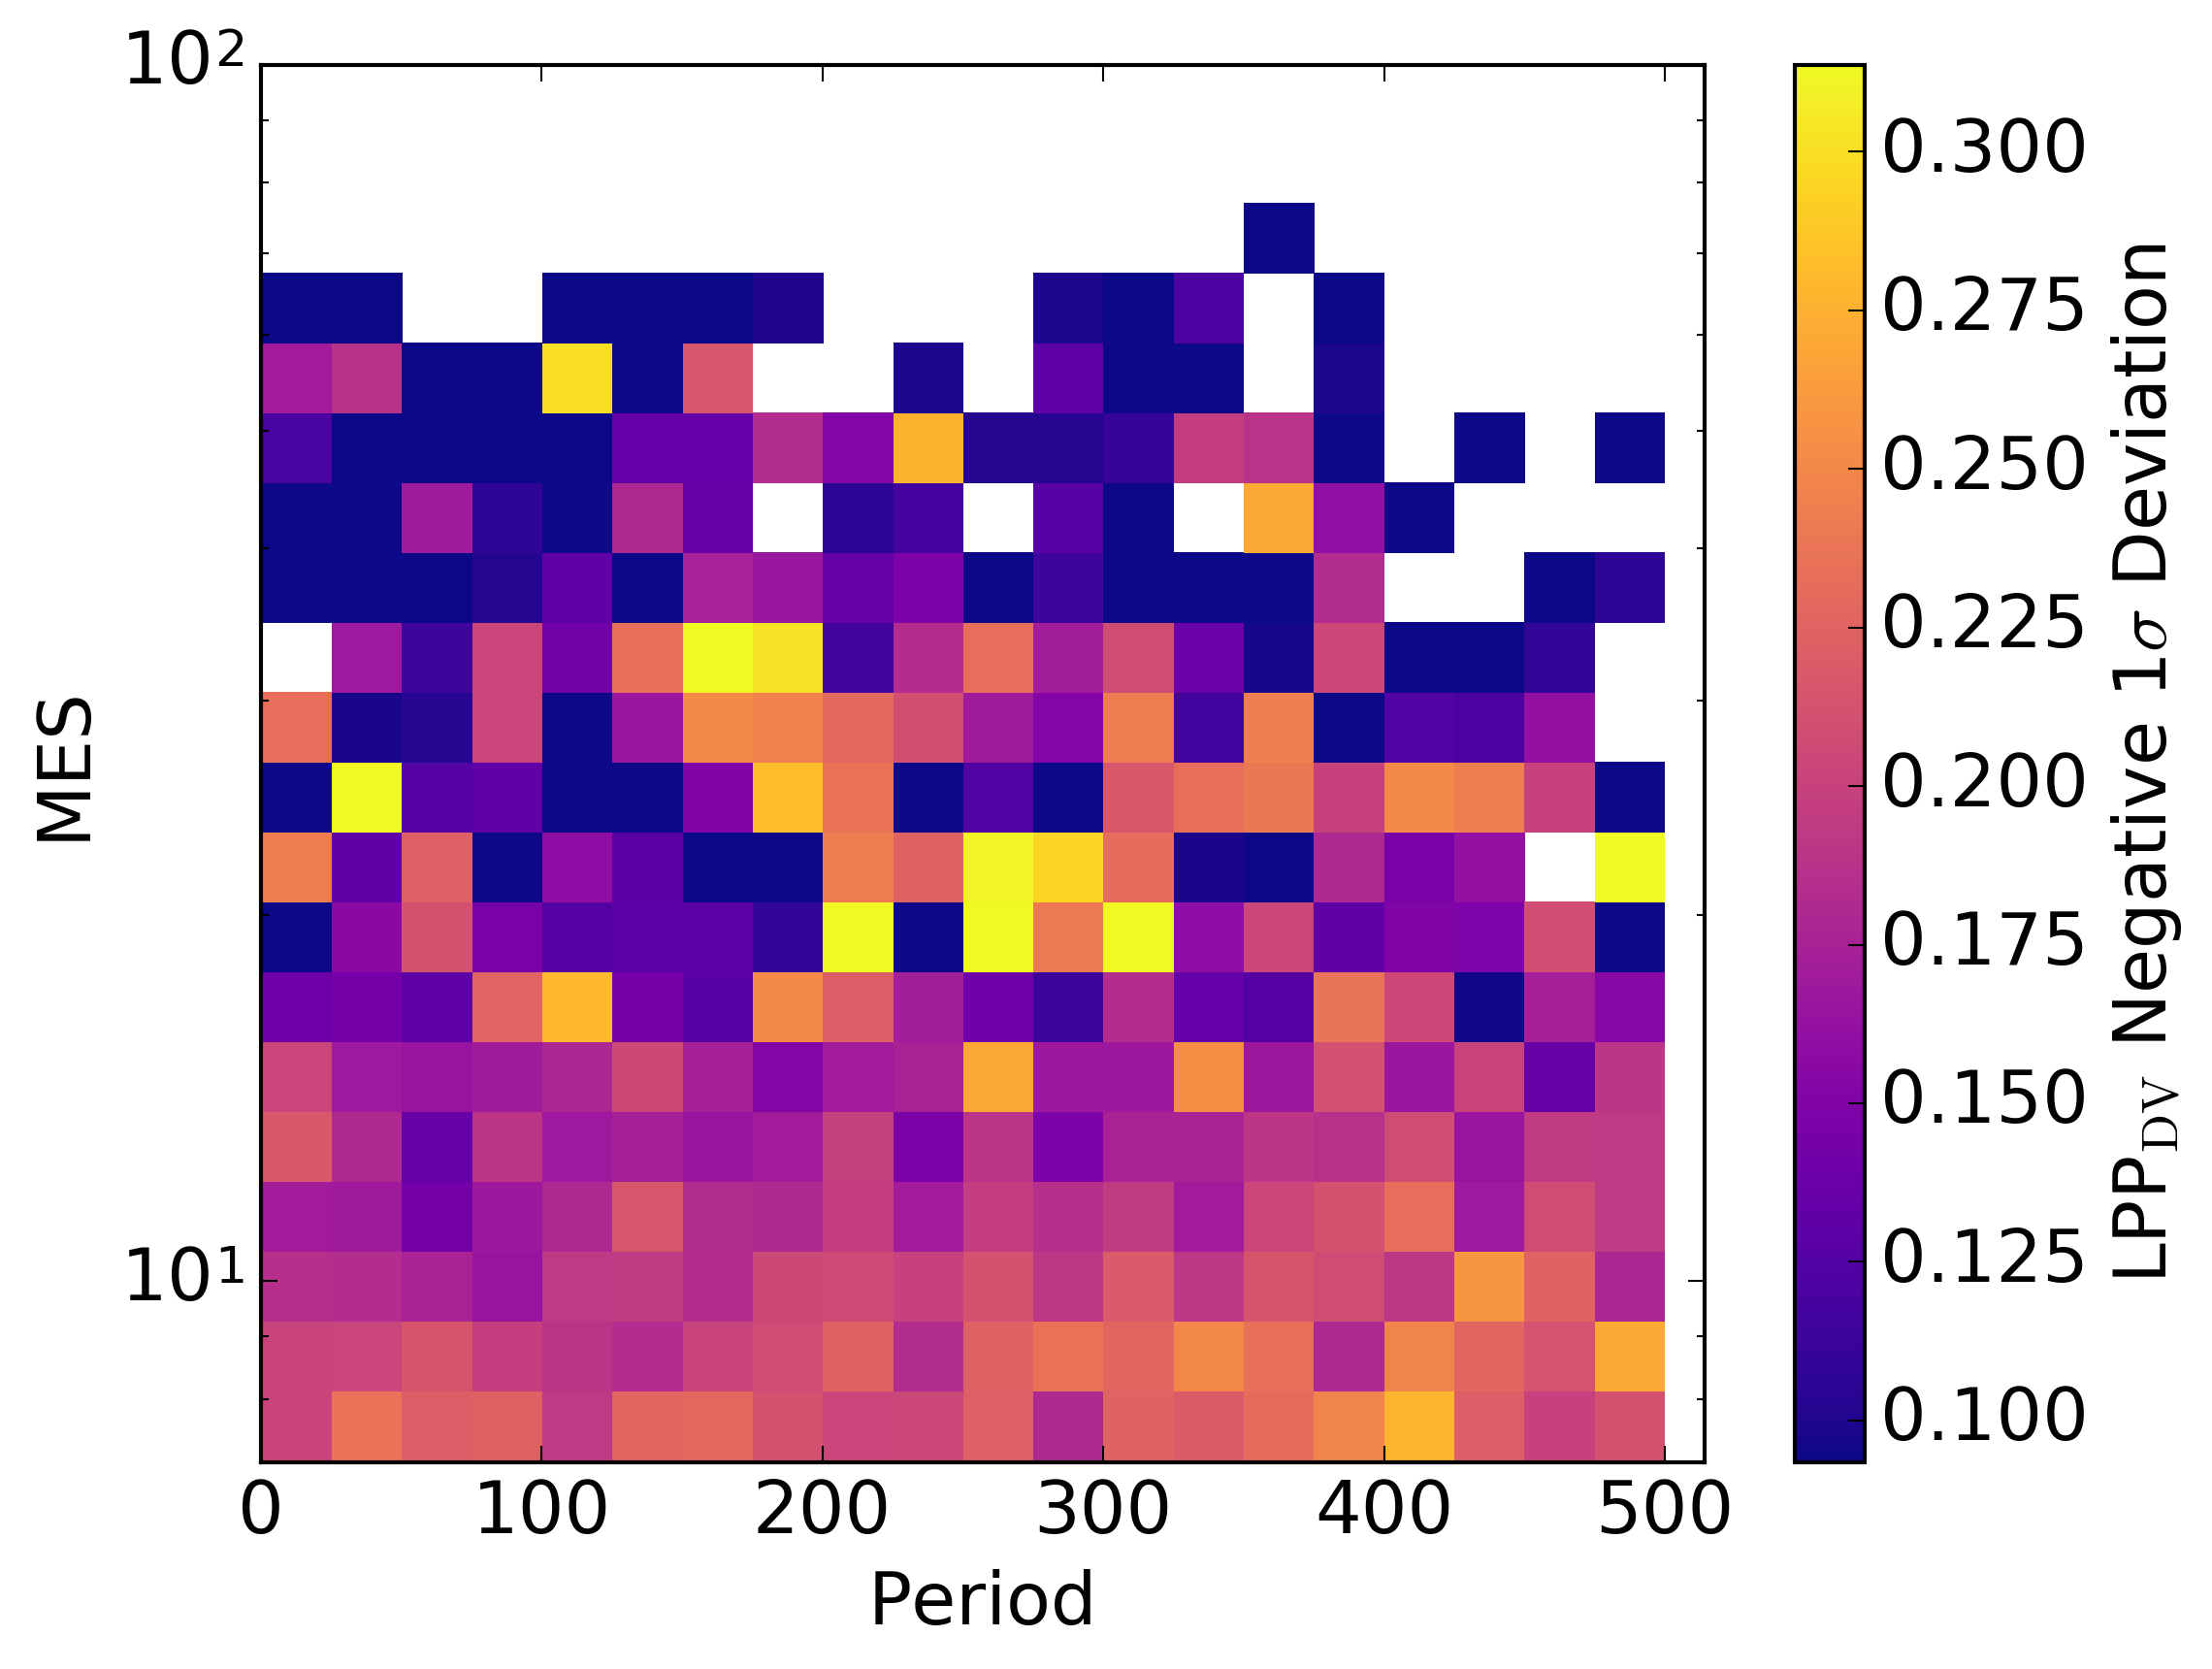
\includegraphics[width=0.5\linewidth]{ScoreFig-5.png} &
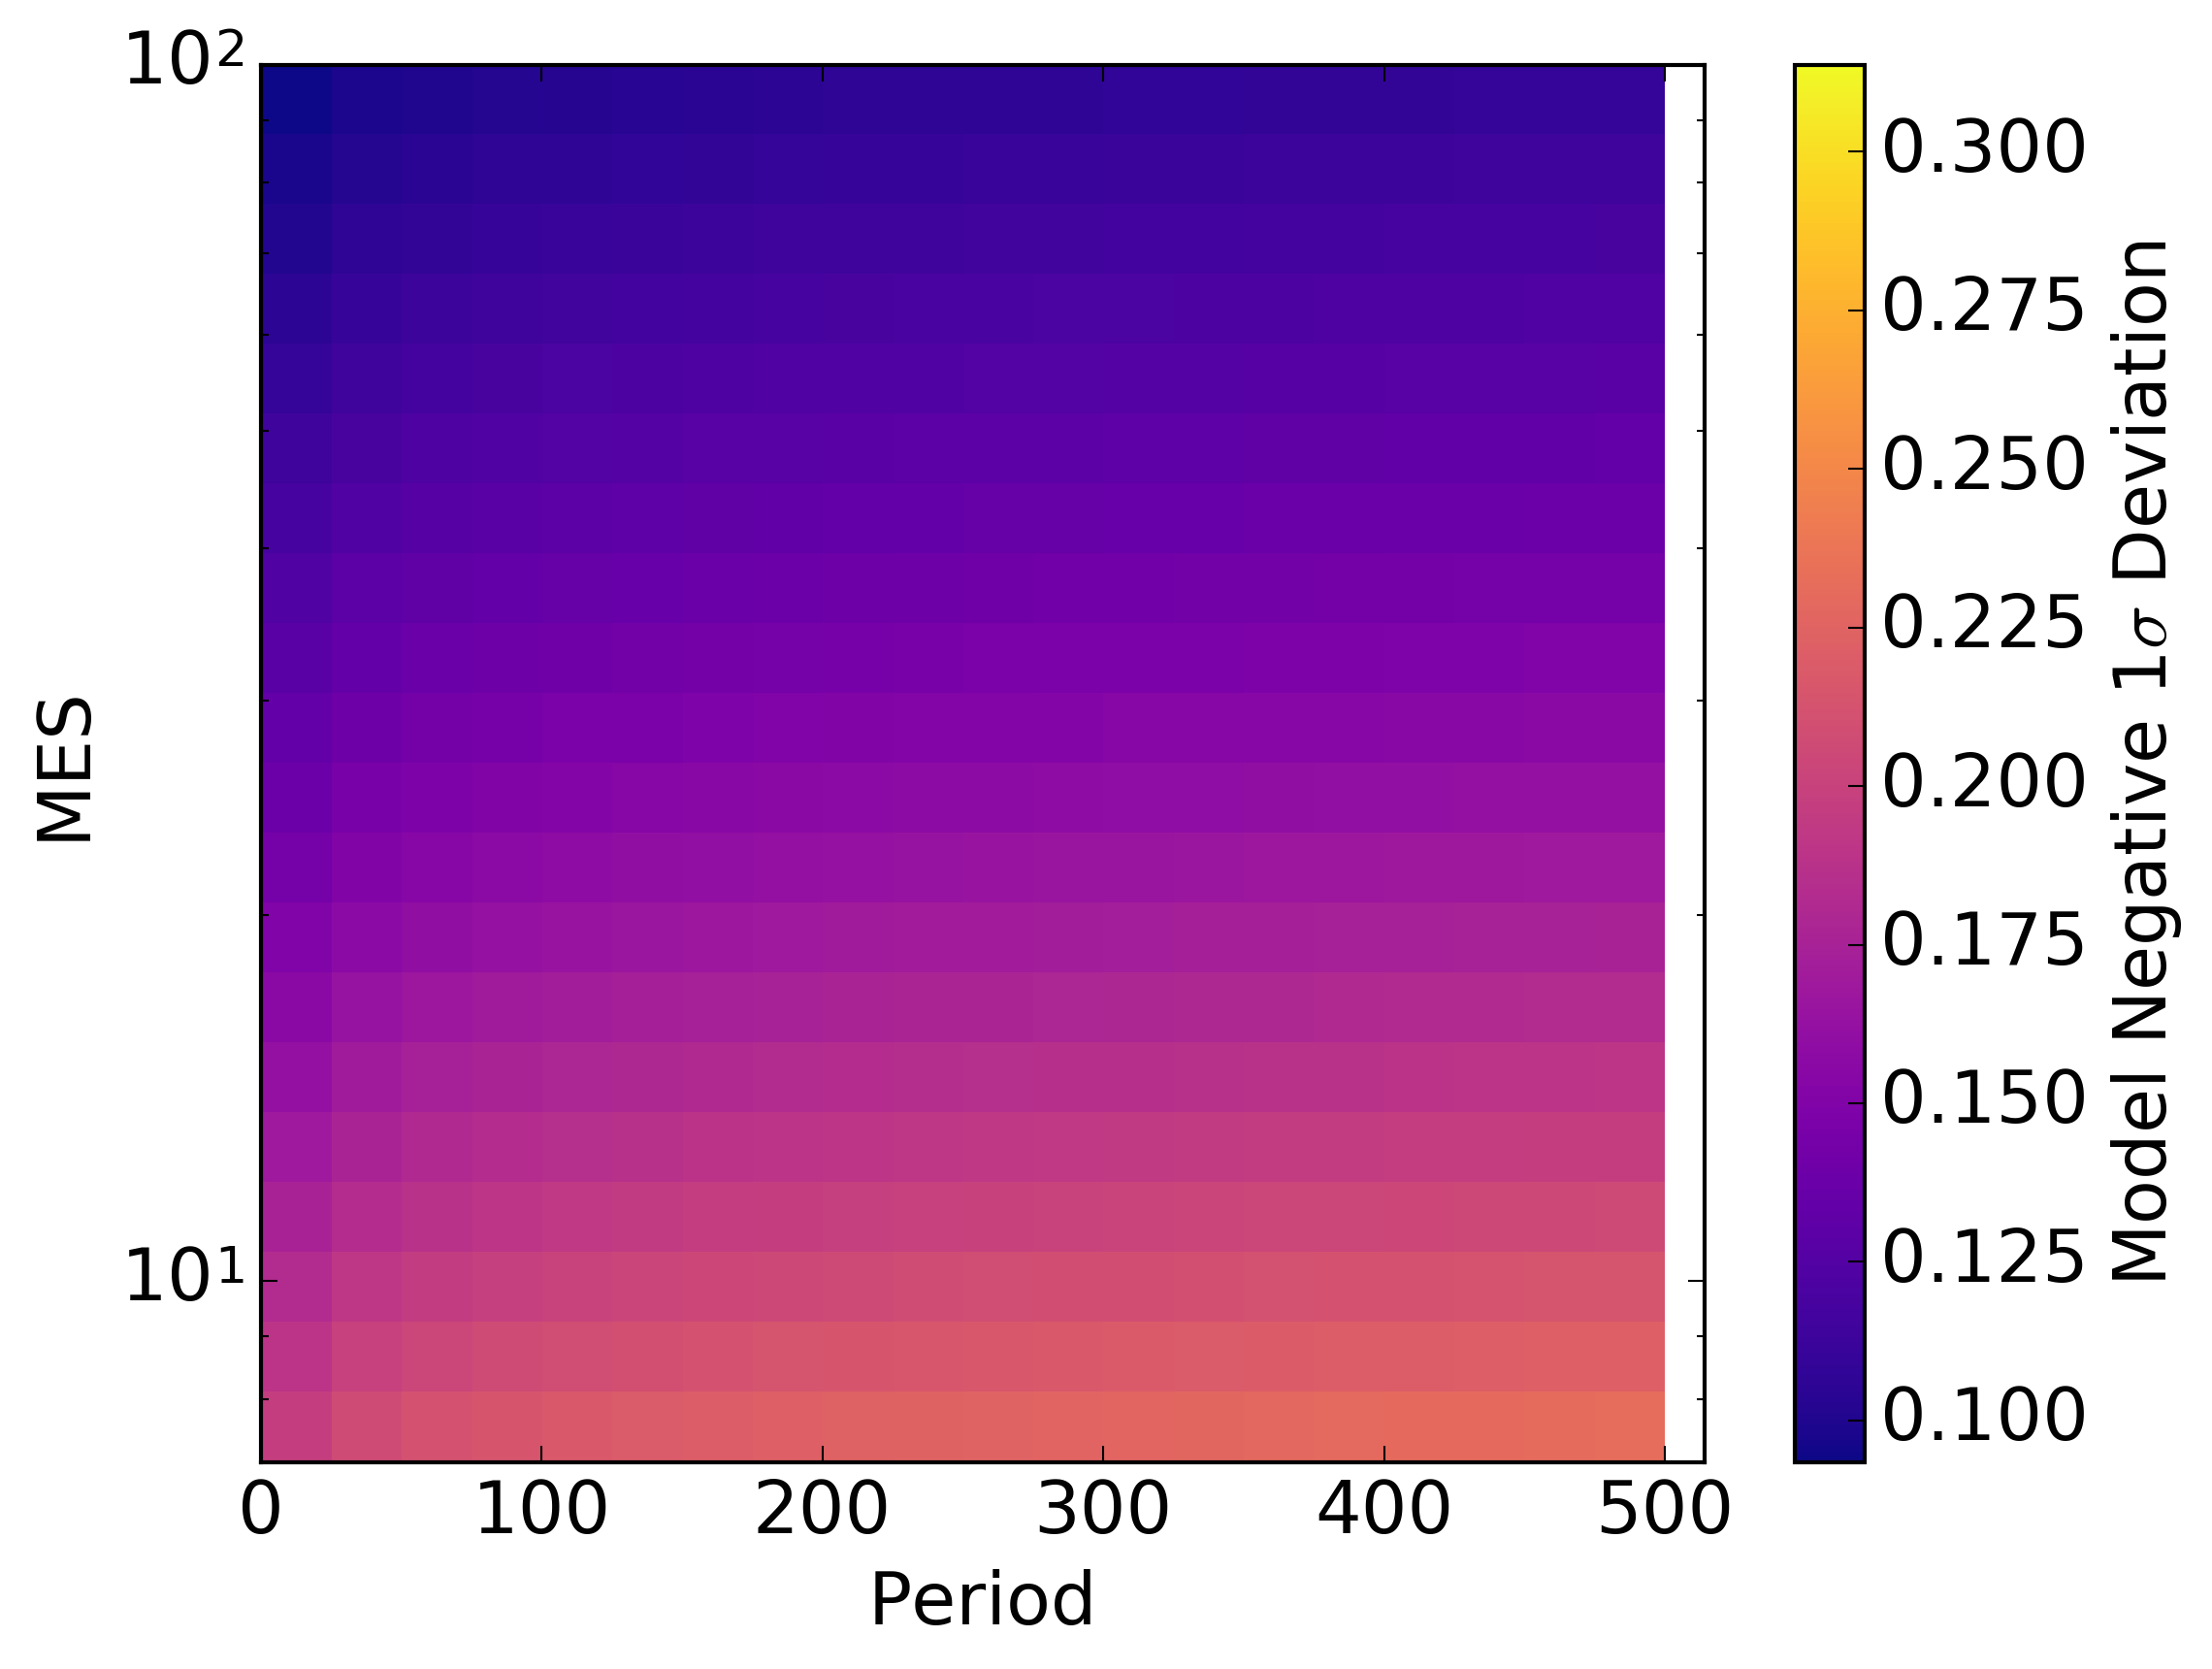
\includegraphics[width=0.5\linewidth]{ScoreFig-6.png}
\end{tabular}
\caption{The top-left plot shows the LPP$_{DV}$ values of all on-target injected planets on FGK dwarf targets as a function of period, and the top-right shows them as a function of MES. The middle-left plots shows the measured positive 1$\sigma$ deviation (in the same units as LPP$_{DV}$) as a function of MES and period, and the middle-right plot shows the resulting best-fit model. The bottom plots show the same thing but for the negative 1$\sigma$ deviation (again in the same units as LPP$_{DV}$). These resulting model distributions are used when computing the Robovetter disposition score.}
\label{score-fig-1}
\end{figure*}
